\documentclass[twoside]{book}

% Packages required by doxygen
\usepackage{calc}
\usepackage{doxygen}
\usepackage{graphicx}
\usepackage[utf8]{inputenc}
\usepackage{makeidx}
\usepackage{multicol}
\usepackage{multirow}
\usepackage{fixltx2e}
\PassOptionsToPackage{warn}{textcomp}
\usepackage{textcomp}
\usepackage[nointegrals]{wasysym}
\usepackage[table]{xcolor}

% Font selection
\usepackage[T1]{fontenc}
\usepackage{mathptmx}
\usepackage[scaled=.90]{helvet}
\usepackage{courier}
\usepackage{amssymb}
\usepackage{sectsty}
\renewcommand{\familydefault}{\sfdefault}
\allsectionsfont{%
  \fontseries{bc}\selectfont%
  \color{darkgray}%
}
\renewcommand{\DoxyLabelFont}{%
  \fontseries{bc}\selectfont%
  \color{darkgray}%
}
\newcommand{\+}{\discretionary{\mbox{\scriptsize$\hookleftarrow$}}{}{}}

% Page & text layout
\usepackage{geometry}
\geometry{%
  a4paper,%
  top=2.5cm,%
  bottom=2.5cm,%
  left=2.5cm,%
  right=2.5cm%
}
\tolerance=750
\hfuzz=15pt
\hbadness=750
\setlength{\emergencystretch}{15pt}
\setlength{\parindent}{0cm}
\setlength{\parskip}{0.2cm}
\makeatletter
\renewcommand{\paragraph}{%
  \@startsection{paragraph}{4}{0ex}{-1.0ex}{1.0ex}{%
    \normalfont\normalsize\bfseries\SS@parafont%
  }%
}
\renewcommand{\subparagraph}{%
  \@startsection{subparagraph}{5}{0ex}{-1.0ex}{1.0ex}{%
    \normalfont\normalsize\bfseries\SS@subparafont%
  }%
}
\makeatother

% Headers & footers
\usepackage{fancyhdr}
\pagestyle{fancyplain}
\fancyhead[LE]{\fancyplain{}{\bfseries\thepage}}
\fancyhead[CE]{\fancyplain{}{}}
\fancyhead[RE]{\fancyplain{}{\bfseries\leftmark}}
\fancyhead[LO]{\fancyplain{}{\bfseries\rightmark}}
\fancyhead[CO]{\fancyplain{}{}}
\fancyhead[RO]{\fancyplain{}{\bfseries\thepage}}
\fancyfoot[LE]{\fancyplain{}{}}
\fancyfoot[CE]{\fancyplain{}{}}
\fancyfoot[RE]{\fancyplain{}{\bfseries\scriptsize Generated on Mon May 5 2014 03\+:03\+:52 for My Project by Doxygen }}
\fancyfoot[LO]{\fancyplain{}{\bfseries\scriptsize Generated on Mon May 5 2014 03\+:03\+:52 for My Project by Doxygen }}
\fancyfoot[CO]{\fancyplain{}{}}
\fancyfoot[RO]{\fancyplain{}{}}
\renewcommand{\footrulewidth}{0.4pt}
\renewcommand{\chaptermark}[1]{%
  \markboth{#1}{}%
}
\renewcommand{\sectionmark}[1]{%
  \markright{\thesection\ #1}%
}

% Indices & bibliography
\usepackage{natbib}
\usepackage[titles]{tocloft}
\setcounter{tocdepth}{3}
\setcounter{secnumdepth}{5}
\makeindex

% Hyperlinks (required, but should be loaded last)
\usepackage{ifpdf}
\ifpdf
  \usepackage[pdftex,pagebackref=true]{hyperref}
\else
  \usepackage[ps2pdf,pagebackref=true]{hyperref}
\fi
\hypersetup{%
  colorlinks=true,%
  linkcolor=blue,%
  citecolor=blue,%
  unicode%
}

% Custom commands
\newcommand{\clearemptydoublepage}{%
  \newpage{\pagestyle{empty}\cleardoublepage}%
}


%===== C O N T E N T S =====

\begin{document}

% Titlepage & ToC
\hypersetup{pageanchor=false,
             bookmarks=true,
             bookmarksnumbered=true,
             pdfencoding=unicode
            }
\pagenumbering{roman}
\begin{titlepage}
\vspace*{7cm}
\begin{center}%
{\Large My Project }\\
\vspace*{1cm}
{\large Generated by Doxygen 1.8.7}\\
\vspace*{0.5cm}
{\small Mon May 5 2014 03:03:52}\\
\end{center}
\end{titlepage}
\clearemptydoublepage
\tableofcontents
\clearemptydoublepage
\pagenumbering{arabic}
\hypersetup{pageanchor=true}

%--- Begin generated contents ---
\chapter{Main Page}
\label{index}\hypertarget{index}{}\hyperlink{class_program}{Program} sluzacy do wyznaczania skutecznosci algorytmu za pomoca pomiaru czasu

Aplikacja jest przykladem realizacji programu sluzacego do sprawdzania zlozonosci obliczeniowej algorytmu. Wykonuje ona pomiar czasu wykonywania zadanego programu. Aplikacja jest zbudowana na obiektach, dzieki czemu mozliwe jest szybkie wstawienie nowego algorytmu w postaci klasy dziedziczacej czesc metod po klasie bazowej.\hypertarget{index_etykieta-wazne-informacje}{}\section{Wazne informacje}\label{index_etykieta-wazne-informacje}
\hyperlink{class_program}{Program} zostal wyposazony w funkcje wczytywania, wypisywania i zapisywania danych do pliku. Aplikacja byla sprawdzana na systemie operacyjnym Windows. Do poprawnego dzialania programu potrzebny jest plik z danymi zapisany w postaci\-: ilosc danych, wlasciwe dane. 
\chapter{Hierarchical Index}
\section{Class Hierarchy}
This inheritance list is sorted roughly, but not completely, alphabetically\-:\begin{DoxyCompactList}
\item \contentsline{section}{benchmark}{\pageref{classbenchmark}}{}
\item \contentsline{section}{Drzewo$<$ typ, klucz, wartosc $>$}{\pageref{class_drzewo}}{}
\item \contentsline{section}{Element$<$ klucz, wartosc $>$}{\pageref{class_element}}{}
\item \contentsline{section}{Komunikacja}{\pageref{class_komunikacja}}{}
\item \contentsline{section}{Program}{\pageref{class_program}}{}
\begin{DoxyCompactList}
\item \contentsline{section}{Przykladowy\-\_\-program}{\pageref{class_przykladowy__program}}{}
\end{DoxyCompactList}
\item \contentsline{section}{Tablica}{\pageref{class_tablica}}{}
\end{DoxyCompactList}

\chapter{Class Index}
\section{Class List}
Here are the classes, structs, unions and interfaces with brief descriptions\+:\begin{DoxyCompactList}
\item\contentsline{section}{\hyperlink{classbenchmark}{benchmark} \\*Klasa benchmarek }{\pageref{classbenchmark}}{}
\item\contentsline{section}{\hyperlink{class_element}{Element$<$ klucz, wartosc $>$} \\*Klasa \hyperlink{class_element}{Element} }{\pageref{class_element}}{}
\item\contentsline{section}{\hyperlink{class_graf}{Graf$<$ krawedz, wierzcholek $>$} \\*Klasa \hyperlink{class_graf}{Graf} }{\pageref{class_graf}}{}
\item\contentsline{section}{\hyperlink{class_komunikacja}{Komunikacja} \\*Klasa \hyperlink{class_komunikacja}{Komunikacja} }{\pageref{class_komunikacja}}{}
\item\contentsline{section}{\hyperlink{class_program}{Program} \\*Klasa \hyperlink{class_program}{Program} }{\pageref{class_program}}{}
\item\contentsline{section}{\hyperlink{class_przykladowy__program}{Przykladowy\+\_\+program} \\*Klasa \hyperlink{class_przykladowy__program}{Przykladowy\+\_\+program} }{\pageref{class_przykladowy__program}}{}
\item\contentsline{section}{\hyperlink{class_tablica}{Tablica} \\*Klasa \hyperlink{class_program}{Program} }{\pageref{class_tablica}}{}
\item\contentsline{section}{\hyperlink{class_tablica__hash}{Tablica\+\_\+hash$<$ typ, klucz, dana $>$} \\*Klasa \hyperlink{class_tablica__hash}{Tablica\+\_\+hash} }{\pageref{class_tablica__hash}}{}
\end{DoxyCompactList}

\chapter{File Index}
\section{File List}
Here is a list of all documented files with brief descriptions\-:\begin{DoxyCompactList}
\item\contentsline{section}{inc/\hyperlink{benchmark_8hh}{benchmark.\-hh} \\*Plik zawierajacy deklaracje klasy benchmark }{\pageref{benchmark_8hh}}{}
\item\contentsline{section}{inc/\hyperlink{mnozenie_8hh}{mnozenie.\-hh} \\*Plik zawierajacy deklaracje klasy \hyperlink{class_mnozenie}{Mnozenie} }{\pageref{mnozenie_8hh}}{}
\item\contentsline{section}{inc/\hyperlink{program_8hh}{program.\-hh} \\*Plik zawierajacy deklaracje klasy \hyperlink{class_program}{Program} }{\pageref{program_8hh}}{}
\item\contentsline{section}{src/\hyperlink{benchmark_8cpp}{benchmark.\-cpp} \\*Plik zawierajacy definicje metod klasy benchmark }{\pageref{benchmark_8cpp}}{}
\item\contentsline{section}{src/\hyperlink{main_8cpp}{main.\-cpp} \\*Plik zawierajacy glowna funkcje programu wykonujacego benchmark algorytmu }{\pageref{main_8cpp}}{}
\item\contentsline{section}{src/\hyperlink{mnozenie_8cpp}{mnozenie.\-cpp} \\*Plik zawierajacy definicje metod klasy \hyperlink{class_mnozenie}{Mnozenie} }{\pageref{mnozenie_8cpp}}{}
\item\contentsline{section}{src/\hyperlink{program_8cpp}{program.\-cpp} \\*Plik zawierajacy definicje metod klasy \hyperlink{class_program}{Program} }{\pageref{program_8cpp}}{}
\end{DoxyCompactList}

\chapter{Class Documentation}
\hypertarget{classbenchmark}{\section{benchmark Class Reference}
\label{classbenchmark}\index{benchmark@{benchmark}}
}


Klasa benchmarek.  




{\ttfamily \#include $<$benchmark.\+hh$>$}

\subsection*{Public Member Functions}
\begin{DoxyCompactItemize}
\item 
bool \hyperlink{classbenchmark_ab83ffeb122d3cc231acdbf45db4f5ff8}{wykonaj\+\_\+sprawdzenie\+\_\+algorytmu} (int ile\+\_\+razy)
\begin{DoxyCompactList}\small\item\em Metoda wykonaj\+\_\+sprawdzenie\+\_\+algorytmu. \end{DoxyCompactList}\item 
double \hyperlink{classbenchmark_a47af0a6ddc3d1e5afe3324f166ae1292}{oblicz\+\_\+sredni\+\_\+czas\+\_\+wykonywania\+\_\+algorytmu} ()
\begin{DoxyCompactList}\small\item\em Metoda oblicz\+\_\+sredni\+\_\+czas\+\_\+wykonywania\+\_\+algorytmu. \end{DoxyCompactList}\item 
\hypertarget{classbenchmark_ad2fa742abac2df08a8a3174ca0cd2a09}{void {\bfseries wypisz\+\_\+tablice\+\_\+czasow} ()}\label{classbenchmark_ad2fa742abac2df08a8a3174ca0cd2a09}

\item 
\hypertarget{classbenchmark_a452c061a57050dacd3429ad5186b49fe}{bool {\bfseries zapisz\+\_\+czasy\+\_\+do\+\_\+pliku} (char $\ast$nazwa)}\label{classbenchmark_a452c061a57050dacd3429ad5186b49fe}

\end{DoxyCompactItemize}


\subsection{Detailed Description}
Klasa benchmarek. 

Klasa wykonujaca sprawdzenie dlugosci wykonywania algorytmu okreslona ilosc razy oraz przedstawienie statystyk zwiazanych z wykonanymi pomiarami. Klasa ta bedzie rozbodowywany w ramach potrzeb przy nastepnych projektach. 

\subsection{Member Function Documentation}
\hypertarget{classbenchmark_a47af0a6ddc3d1e5afe3324f166ae1292}{\index{benchmark@{benchmark}!oblicz\+\_\+sredni\+\_\+czas\+\_\+wykonywania\+\_\+algorytmu@{oblicz\+\_\+sredni\+\_\+czas\+\_\+wykonywania\+\_\+algorytmu}}
\index{oblicz\+\_\+sredni\+\_\+czas\+\_\+wykonywania\+\_\+algorytmu@{oblicz\+\_\+sredni\+\_\+czas\+\_\+wykonywania\+\_\+algorytmu}!benchmark@{benchmark}}
\subsubsection[{oblicz\+\_\+sredni\+\_\+czas\+\_\+wykonywania\+\_\+algorytmu}]{\setlength{\rightskip}{0pt plus 5cm}double benchmark\+::oblicz\+\_\+sredni\+\_\+czas\+\_\+wykonywania\+\_\+algorytmu (
\begin{DoxyParamCaption}
{}
\end{DoxyParamCaption}
)}}\label{classbenchmark_a47af0a6ddc3d1e5afe3324f166ae1292}


Metoda oblicz\+\_\+sredni\+\_\+czas\+\_\+wykonywania\+\_\+algorytmu. 

\begin{DoxyReturn}{Returns}
Zwraca wartosc srednia potrzebna na wykonanie algorytmu w sekundach (liczba double). 
\end{DoxyReturn}
\hypertarget{classbenchmark_ab83ffeb122d3cc231acdbf45db4f5ff8}{\index{benchmark@{benchmark}!wykonaj\+\_\+sprawdzenie\+\_\+algorytmu@{wykonaj\+\_\+sprawdzenie\+\_\+algorytmu}}
\index{wykonaj\+\_\+sprawdzenie\+\_\+algorytmu@{wykonaj\+\_\+sprawdzenie\+\_\+algorytmu}!benchmark@{benchmark}}
\subsubsection[{wykonaj\+\_\+sprawdzenie\+\_\+algorytmu}]{\setlength{\rightskip}{0pt plus 5cm}bool benchmark\+::wykonaj\+\_\+sprawdzenie\+\_\+algorytmu (
\begin{DoxyParamCaption}
\item[{int}]{ile\+\_\+razy}
\end{DoxyParamCaption}
)}}\label{classbenchmark_ab83ffeb122d3cc231acdbf45db4f5ff8}


Metoda wykonaj\+\_\+sprawdzenie\+\_\+algorytmu. 


\begin{DoxyParams}[1]{Parameters}
\mbox{\tt in}  & {\em Ilosc} & wykonan algorytmu. \\
\hline
\end{DoxyParams}


The documentation for this class was generated from the following files\+:\begin{DoxyCompactItemize}
\item 
inc/\hyperlink{benchmark_8hh}{benchmark.\+hh}\item 
src/\hyperlink{benchmark_8cpp}{benchmark.\+cpp}\end{DoxyCompactItemize}

\hypertarget{class_element}{\section{Element$<$ klucz, wartosc $>$ Class Template Reference}
\label{class_element}\index{Element$<$ klucz, wartosc $>$@{Element$<$ klucz, wartosc $>$}}
}


Klasa \hyperlink{class_element}{Element}.  




{\ttfamily \#include $<$element.\+hh$>$}

\subsection*{Public Member Functions}
\begin{DoxyCompactItemize}
\item 
\hyperlink{class_element_a2908ce7965da27acf29ba7a8ed702a9e}{Element} ()
\begin{DoxyCompactList}\small\item\em Konstruktor \hyperlink{class_element}{Element}. \end{DoxyCompactList}\item 
wartosc $\ast$ \hyperlink{class_element_a95e99b08207e2eee854855a3cf624ee8}{wpisz\+\_\+wartosc} (wartosc $\ast$dana)
\begin{DoxyCompactList}\small\item\em Metoda wpisz\+\_\+wartosc. \end{DoxyCompactList}\item 
void \hyperlink{class_element_aab83ecbc43e50357b34839a7836f7f00}{wpisz\+\_\+klucz} (klucz haslo)
\begin{DoxyCompactList}\small\item\em Metoda wpisz\+\_\+klucz. \end{DoxyCompactList}\item 
void \hyperlink{class_element_aea3e8d9929eaf9921ba3e805ccae9d3c}{wpisz\+\_\+klucz2} (klucz haslo)
\begin{DoxyCompactList}\small\item\em Metoda wpisz\+\_\+klucz. \end{DoxyCompactList}\item 
int \hyperlink{class_element_afb6bb7f1f9c6a127b66bd8a49f83f1dc}{wpisz\+\_\+wage} (int waga)
\begin{DoxyCompactList}\small\item\em wpisz\+\_\+wage \end{DoxyCompactList}\item 
void \hyperlink{class_element_a9d169d81af34f308bc80b6fdcc87e139}{wpisz\+\_\+ojciec} (\hyperlink{class_element}{Element}$<$ klucz, wartosc $>$ $\ast$wskaznik)
\begin{DoxyCompactList}\small\item\em Metoda wpisz\+\_\+ojciec. \end{DoxyCompactList}\item 
void \hyperlink{class_element_ac2dd0d138001f2de876f306b83298914}{wpisz\+\_\+wskaznik} (\hyperlink{class_element}{Element}$<$ klucz, wartosc $>$ $\ast$wskaznik)
\begin{DoxyCompactList}\small\item\em Metoda wpisz\+\_\+wskaznik. \end{DoxyCompactList}\item 
wartosc $\ast$ \hyperlink{class_element_a1cfca5911c61ac275fd60c9d9c173b6d}{zwroc\+\_\+wartosc} ()
\begin{DoxyCompactList}\small\item\em Metoda zwroc\+\_\+wartosc. \end{DoxyCompactList}\item 
int \hyperlink{class_element_a748fcfad2139d088fd7f612578663909}{zwroc\+\_\+wage} ()
\begin{DoxyCompactList}\small\item\em Metoda zwroc\+\_\+wage. \end{DoxyCompactList}\item 
klucz \hyperlink{class_element_a4041559698851d33d77d9c457f3a5da4}{zwroc\+\_\+klucz} ()
\begin{DoxyCompactList}\small\item\em Metoda zwroc\+\_\+klucz. \end{DoxyCompactList}\item 
klucz \hyperlink{class_element_a432a0f6d8a5291051644667a39a3c1ba}{zwroc\+\_\+klucz2} ()
\begin{DoxyCompactList}\small\item\em Metoda zwroc\+\_\+klucz2. \end{DoxyCompactList}\item 
\hyperlink{class_element}{Element} $\ast$ \hyperlink{class_element_acee0fb7c5bbe330961d16e6e672d07d2}{zwroc\+\_\+wskaznik} ()
\begin{DoxyCompactList}\small\item\em Metoda zwroc\+\_\+wskaznik. \end{DoxyCompactList}\item 
\hyperlink{class_element}{Element} $\ast$ \hyperlink{class_element_ac24b7bfe84763613a838012e85ad4ac4}{zwroc\+\_\+ojciec} ()
\begin{DoxyCompactList}\small\item\em Metoda zwroc\+\_\+ojciec. \end{DoxyCompactList}\item 
void \hyperlink{class_element_aacd6653f0fa6475a8b2e122dddf80627}{przepisz\+\_\+dane} (\hyperlink{class_element}{Element}$<$ klucz, wartosc $>$ $\ast$wskaznik)
\begin{DoxyCompactList}\small\item\em Metoda przepisz\+\_\+dane. \end{DoxyCompactList}\item 
bool \hyperlink{class_element_a92f1c6c72a7b768cd2d295eb6b6c3d0e}{czy\+\_\+odwiedzony} ()
\begin{DoxyCompactList}\small\item\em czy\+\_\+odwiedzony \end{DoxyCompactList}\item 
void \hyperlink{class_element_af45d4a7953e01a1d9916eed0ab17f6bb}{odwiedzony} ()
\begin{DoxyCompactList}\small\item\em odwiedzony \end{DoxyCompactList}\item 
void \hyperlink{class_element_a1091b5a9763464470901903c27fa3af4}{nie\+\_\+odwiedzony} ()
\begin{DoxyCompactList}\small\item\em nie\+\_\+odwiedzony \end{DoxyCompactList}\item 
void \hyperlink{class_element_aea8ebe54afa2525740e1b065f9fd3a13}{sasiedzi\+\_\+odwiedzeni} ()
\begin{DoxyCompactList}\small\item\em sasiedzi\+\_\+odwiedzeni \end{DoxyCompactList}\item 
void \hyperlink{class_element_a04d9f1bebfc82dad1ca3e32e1f84fd5d}{sasiedzi\+\_\+nie\+\_\+odwiedzeni} ()
\begin{DoxyCompactList}\small\item\em sasiedzi\+\_\+nie\+\_\+odwiedzeni \end{DoxyCompactList}\item 
bool \hyperlink{class_element_a07619a03996d2a7261d78dea30319d7a}{czy\+\_\+sasiedzi\+\_\+odwiedzeni} ()
\begin{DoxyCompactList}\small\item\em sasiedzi\+\_\+odwiedzeni \end{DoxyCompactList}\item 
void \hyperlink{class_element_afd6003b54275449e8b67d34a842a87fc}{wypisz} ()
\begin{DoxyCompactList}\small\item\em wypisz \end{DoxyCompactList}\end{DoxyCompactItemize}


\subsection{Detailed Description}
\subsubsection*{template$<$class klucz, class wartosc$>$class Element$<$ klucz, wartosc $>$}

Klasa \hyperlink{class_element}{Element}. 

Klasa przechowuje dane oraz klucze po ktorych odbywa sie szukanie danych. Klasa jest przystosowana do wokorzystania jako element grafu wiec zawiera wskazniki oraz metody potrzebne do polaczenia z innymi elementami. 

\subsection{Constructor \& Destructor Documentation}
\hypertarget{class_element_a2908ce7965da27acf29ba7a8ed702a9e}{\index{Element@{Element}!Element@{Element}}
\index{Element@{Element}!Element@{Element}}
\subsubsection[{Element}]{\setlength{\rightskip}{0pt plus 5cm}template$<$class klucz, class wartosc$>$ {\bf Element}$<$ klucz, wartosc $>$\+::{\bf Element} (
\begin{DoxyParamCaption}
{}
\end{DoxyParamCaption}
)\hspace{0.3cm}{\ttfamily [inline]}}}\label{class_element_a2908ce7965da27acf29ba7a8ed702a9e}


Konstruktor \hyperlink{class_element}{Element}. 

Ustawia wskazniki na N\+U\+L\+L. 

\subsection{Member Function Documentation}
\hypertarget{class_element_a92f1c6c72a7b768cd2d295eb6b6c3d0e}{\index{Element@{Element}!czy\+\_\+odwiedzony@{czy\+\_\+odwiedzony}}
\index{czy\+\_\+odwiedzony@{czy\+\_\+odwiedzony}!Element@{Element}}
\subsubsection[{czy\+\_\+odwiedzony}]{\setlength{\rightskip}{0pt plus 5cm}template$<$class klucz, class wartosc$>$ bool {\bf Element}$<$ klucz, wartosc $>$\+::czy\+\_\+odwiedzony (
\begin{DoxyParamCaption}
{}
\end{DoxyParamCaption}
)\hspace{0.3cm}{\ttfamily [inline]}}}\label{class_element_a92f1c6c72a7b768cd2d295eb6b6c3d0e}


czy\+\_\+odwiedzony 

\begin{DoxyReturn}{Returns}
Metoda zwracajaca informacje o tym czy dany element zostal odwiedzony. (czy w polu odwiedzony znajduje sie wartosc true) 
\end{DoxyReturn}
\hypertarget{class_element_a07619a03996d2a7261d78dea30319d7a}{\index{Element@{Element}!czy\+\_\+sasiedzi\+\_\+odwiedzeni@{czy\+\_\+sasiedzi\+\_\+odwiedzeni}}
\index{czy\+\_\+sasiedzi\+\_\+odwiedzeni@{czy\+\_\+sasiedzi\+\_\+odwiedzeni}!Element@{Element}}
\subsubsection[{czy\+\_\+sasiedzi\+\_\+odwiedzeni}]{\setlength{\rightskip}{0pt plus 5cm}template$<$class klucz, class wartosc$>$ bool {\bf Element}$<$ klucz, wartosc $>$\+::czy\+\_\+sasiedzi\+\_\+odwiedzeni (
\begin{DoxyParamCaption}
{}
\end{DoxyParamCaption}
)\hspace{0.3cm}{\ttfamily [inline]}}}\label{class_element_a07619a03996d2a7261d78dea30319d7a}


sasiedzi\+\_\+odwiedzeni 

Metoda zwracajaca informacje czy sasiedzi elementu zostali odwiedzeni. (zwracana jest wartosc pola \+\_\+sasiedzi\+\_\+odwiedzeni) \hypertarget{class_element_a1091b5a9763464470901903c27fa3af4}{\index{Element@{Element}!nie\+\_\+odwiedzony@{nie\+\_\+odwiedzony}}
\index{nie\+\_\+odwiedzony@{nie\+\_\+odwiedzony}!Element@{Element}}
\subsubsection[{nie\+\_\+odwiedzony}]{\setlength{\rightskip}{0pt plus 5cm}template$<$class klucz, class wartosc$>$ void {\bf Element}$<$ klucz, wartosc $>$\+::nie\+\_\+odwiedzony (
\begin{DoxyParamCaption}
{}
\end{DoxyParamCaption}
)\hspace{0.3cm}{\ttfamily [inline]}}}\label{class_element_a1091b5a9763464470901903c27fa3af4}


nie\+\_\+odwiedzony 

Metoda wpisujaca od zmiennej \+\_\+odwiedzony wartosc false. \hypertarget{class_element_af45d4a7953e01a1d9916eed0ab17f6bb}{\index{Element@{Element}!odwiedzony@{odwiedzony}}
\index{odwiedzony@{odwiedzony}!Element@{Element}}
\subsubsection[{odwiedzony}]{\setlength{\rightskip}{0pt plus 5cm}template$<$class klucz, class wartosc$>$ void {\bf Element}$<$ klucz, wartosc $>$\+::odwiedzony (
\begin{DoxyParamCaption}
{}
\end{DoxyParamCaption}
)\hspace{0.3cm}{\ttfamily [inline]}}}\label{class_element_af45d4a7953e01a1d9916eed0ab17f6bb}


odwiedzony 

Metoda wpisujaca do zmiennej \+\_\+odwiedzony wartosc true. \hypertarget{class_element_aacd6653f0fa6475a8b2e122dddf80627}{\index{Element@{Element}!przepisz\+\_\+dane@{przepisz\+\_\+dane}}
\index{przepisz\+\_\+dane@{przepisz\+\_\+dane}!Element@{Element}}
\subsubsection[{przepisz\+\_\+dane}]{\setlength{\rightskip}{0pt plus 5cm}template$<$class klucz, class wartosc$>$ void {\bf Element}$<$ klucz, wartosc $>$\+::przepisz\+\_\+dane (
\begin{DoxyParamCaption}
\item[{{\bf Element}$<$ klucz, wartosc $>$ $\ast$}]{wskaznik}
\end{DoxyParamCaption}
)}}\label{class_element_aacd6653f0fa6475a8b2e122dddf80627}


Metoda przepisz\+\_\+dane. 

Metoda przepisujaca same dane bez zmiany wskaznikow. \hypertarget{class_element_a04d9f1bebfc82dad1ca3e32e1f84fd5d}{\index{Element@{Element}!sasiedzi\+\_\+nie\+\_\+odwiedzeni@{sasiedzi\+\_\+nie\+\_\+odwiedzeni}}
\index{sasiedzi\+\_\+nie\+\_\+odwiedzeni@{sasiedzi\+\_\+nie\+\_\+odwiedzeni}!Element@{Element}}
\subsubsection[{sasiedzi\+\_\+nie\+\_\+odwiedzeni}]{\setlength{\rightskip}{0pt plus 5cm}template$<$class klucz, class wartosc$>$ void {\bf Element}$<$ klucz, wartosc $>$\+::sasiedzi\+\_\+nie\+\_\+odwiedzeni (
\begin{DoxyParamCaption}
{}
\end{DoxyParamCaption}
)\hspace{0.3cm}{\ttfamily [inline]}}}\label{class_element_a04d9f1bebfc82dad1ca3e32e1f84fd5d}


sasiedzi\+\_\+nie\+\_\+odwiedzeni 

Metoda wpisujaca wartosc false do zmiennej sasiedzi\+\_\+odwiedzeni. \hypertarget{class_element_aea8ebe54afa2525740e1b065f9fd3a13}{\index{Element@{Element}!sasiedzi\+\_\+odwiedzeni@{sasiedzi\+\_\+odwiedzeni}}
\index{sasiedzi\+\_\+odwiedzeni@{sasiedzi\+\_\+odwiedzeni}!Element@{Element}}
\subsubsection[{sasiedzi\+\_\+odwiedzeni}]{\setlength{\rightskip}{0pt plus 5cm}template$<$class klucz, class wartosc$>$ void {\bf Element}$<$ klucz, wartosc $>$\+::sasiedzi\+\_\+odwiedzeni (
\begin{DoxyParamCaption}
{}
\end{DoxyParamCaption}
)\hspace{0.3cm}{\ttfamily [inline]}}}\label{class_element_aea8ebe54afa2525740e1b065f9fd3a13}


sasiedzi\+\_\+odwiedzeni 

Metoda wpisujaca wartosc true do zmiennej sasiedzi\+\_\+odwiedzeni. \hypertarget{class_element_aab83ecbc43e50357b34839a7836f7f00}{\index{Element@{Element}!wpisz\+\_\+klucz@{wpisz\+\_\+klucz}}
\index{wpisz\+\_\+klucz@{wpisz\+\_\+klucz}!Element@{Element}}
\subsubsection[{wpisz\+\_\+klucz}]{\setlength{\rightskip}{0pt plus 5cm}template$<$class klucz, class wartosc$>$ void {\bf Element}$<$ klucz, wartosc $>$\+::wpisz\+\_\+klucz (
\begin{DoxyParamCaption}
\item[{klucz}]{haslo}
\end{DoxyParamCaption}
)\hspace{0.3cm}{\ttfamily [inline]}}}\label{class_element_aab83ecbc43e50357b34839a7836f7f00}


Metoda wpisz\+\_\+klucz. 


\begin{DoxyParams}[1]{Parameters}
\mbox{\tt in}  & {\em haslo} & Metoda wpisujaca klucz po ktorym mozna znalezc element. \\
\hline
\end{DoxyParams}
\hypertarget{class_element_aea3e8d9929eaf9921ba3e805ccae9d3c}{\index{Element@{Element}!wpisz\+\_\+klucz2@{wpisz\+\_\+klucz2}}
\index{wpisz\+\_\+klucz2@{wpisz\+\_\+klucz2}!Element@{Element}}
\subsubsection[{wpisz\+\_\+klucz2}]{\setlength{\rightskip}{0pt plus 5cm}template$<$class klucz, class wartosc$>$ void {\bf Element}$<$ klucz, wartosc $>$\+::wpisz\+\_\+klucz2 (
\begin{DoxyParamCaption}
\item[{klucz}]{haslo}
\end{DoxyParamCaption}
)\hspace{0.3cm}{\ttfamily [inline]}}}\label{class_element_aea3e8d9929eaf9921ba3e805ccae9d3c}


Metoda wpisz\+\_\+klucz. 


\begin{DoxyParams}[1]{Parameters}
\mbox{\tt in}  & {\em haslo2} & Metoda wpisujaca klucz po ktorym mozna znalezc element. \\
\hline
\end{DoxyParams}
\hypertarget{class_element_a9d169d81af34f308bc80b6fdcc87e139}{\index{Element@{Element}!wpisz\+\_\+ojciec@{wpisz\+\_\+ojciec}}
\index{wpisz\+\_\+ojciec@{wpisz\+\_\+ojciec}!Element@{Element}}
\subsubsection[{wpisz\+\_\+ojciec}]{\setlength{\rightskip}{0pt plus 5cm}template$<$class klucz, class wartosc$>$ void {\bf Element}$<$ klucz, wartosc $>$\+::wpisz\+\_\+ojciec (
\begin{DoxyParamCaption}
\item[{{\bf Element}$<$ klucz, wartosc $>$ $\ast$}]{wskaznik}
\end{DoxyParamCaption}
)\hspace{0.3cm}{\ttfamily [inline]}}}\label{class_element_a9d169d81af34f308bc80b6fdcc87e139}


Metoda wpisz\+\_\+ojciec. 


\begin{DoxyParams}[1]{Parameters}
\mbox{\tt in}  & {\em } & do odpowiedniej struktury. Wpisuje wskaznik do struktury typu \hyperlink{class_element}{Element}. \\
\hline
\end{DoxyParams}
\hypertarget{class_element_afb6bb7f1f9c6a127b66bd8a49f83f1dc}{\index{Element@{Element}!wpisz\+\_\+wage@{wpisz\+\_\+wage}}
\index{wpisz\+\_\+wage@{wpisz\+\_\+wage}!Element@{Element}}
\subsubsection[{wpisz\+\_\+wage}]{\setlength{\rightskip}{0pt plus 5cm}template$<$class klucz, class wartosc$>$ int {\bf Element}$<$ klucz, wartosc $>$\+::wpisz\+\_\+wage (
\begin{DoxyParamCaption}
\item[{int}]{waga}
\end{DoxyParamCaption}
)\hspace{0.3cm}{\ttfamily [inline]}}}\label{class_element_afb6bb7f1f9c6a127b66bd8a49f83f1dc}


wpisz\+\_\+wage 

Metoda wpisujaca wage do elementu. \hypertarget{class_element_a95e99b08207e2eee854855a3cf624ee8}{\index{Element@{Element}!wpisz\+\_\+wartosc@{wpisz\+\_\+wartosc}}
\index{wpisz\+\_\+wartosc@{wpisz\+\_\+wartosc}!Element@{Element}}
\subsubsection[{wpisz\+\_\+wartosc}]{\setlength{\rightskip}{0pt plus 5cm}template$<$class klucz, class wartosc$>$ wartosc$\ast$ {\bf Element}$<$ klucz, wartosc $>$\+::wpisz\+\_\+wartosc (
\begin{DoxyParamCaption}
\item[{wartosc $\ast$}]{dana}
\end{DoxyParamCaption}
)\hspace{0.3cm}{\ttfamily [inline]}}}\label{class_element_a95e99b08207e2eee854855a3cf624ee8}


Metoda wpisz\+\_\+wartosc. 


\begin{DoxyParams}[1]{Parameters}
\mbox{\tt in}  & {\em dana} & Metoda wpisujaca wartosc do zmiennej zawierajacej dane elementu. \\
\hline
\end{DoxyParams}
\hypertarget{class_element_ac2dd0d138001f2de876f306b83298914}{\index{Element@{Element}!wpisz\+\_\+wskaznik@{wpisz\+\_\+wskaznik}}
\index{wpisz\+\_\+wskaznik@{wpisz\+\_\+wskaznik}!Element@{Element}}
\subsubsection[{wpisz\+\_\+wskaznik}]{\setlength{\rightskip}{0pt plus 5cm}template$<$class klucz, class wartosc$>$ void {\bf Element}$<$ klucz, wartosc $>$\+::wpisz\+\_\+wskaznik (
\begin{DoxyParamCaption}
\item[{{\bf Element}$<$ klucz, wartosc $>$ $\ast$}]{wskaznik}
\end{DoxyParamCaption}
)\hspace{0.3cm}{\ttfamily [inline]}}}\label{class_element_ac2dd0d138001f2de876f306b83298914}


Metoda wpisz\+\_\+wskaznik. 


\begin{DoxyParams}[1]{Parameters}
\mbox{\tt in}  & {\em } & do odpowiedniej struktury. Wpisuje wskaznik do struktury typu \hyperlink{class_element}{Element}. \\
\hline
\end{DoxyParams}
\hypertarget{class_element_afd6003b54275449e8b67d34a842a87fc}{\index{Element@{Element}!wypisz@{wypisz}}
\index{wypisz@{wypisz}!Element@{Element}}
\subsubsection[{wypisz}]{\setlength{\rightskip}{0pt plus 5cm}template$<$class klucz , class wartosc $>$ void {\bf Element}$<$ klucz, wartosc $>$\+::wypisz (
\begin{DoxyParamCaption}
{}
\end{DoxyParamCaption}
)}}\label{class_element_afd6003b54275449e8b67d34a842a87fc}


wypisz 

Metoda wypisujaca element. Na std out zostaja wypisane klucze oraz waga. \hypertarget{class_element_a4041559698851d33d77d9c457f3a5da4}{\index{Element@{Element}!zwroc\+\_\+klucz@{zwroc\+\_\+klucz}}
\index{zwroc\+\_\+klucz@{zwroc\+\_\+klucz}!Element@{Element}}
\subsubsection[{zwroc\+\_\+klucz}]{\setlength{\rightskip}{0pt plus 5cm}template$<$class klucz, class wartosc$>$ klucz {\bf Element}$<$ klucz, wartosc $>$\+::zwroc\+\_\+klucz (
\begin{DoxyParamCaption}
{}
\end{DoxyParamCaption}
)\hspace{0.3cm}{\ttfamily [inline]}}}\label{class_element_a4041559698851d33d77d9c457f3a5da4}


Metoda zwroc\+\_\+klucz. 

\begin{DoxyReturn}{Returns}
Metoda zwracajaca klucz po ktorym odbywa sie szukanie. 
\end{DoxyReturn}
\hypertarget{class_element_a432a0f6d8a5291051644667a39a3c1ba}{\index{Element@{Element}!zwroc\+\_\+klucz2@{zwroc\+\_\+klucz2}}
\index{zwroc\+\_\+klucz2@{zwroc\+\_\+klucz2}!Element@{Element}}
\subsubsection[{zwroc\+\_\+klucz2}]{\setlength{\rightskip}{0pt plus 5cm}template$<$class klucz, class wartosc$>$ klucz {\bf Element}$<$ klucz, wartosc $>$\+::zwroc\+\_\+klucz2 (
\begin{DoxyParamCaption}
{}
\end{DoxyParamCaption}
)\hspace{0.3cm}{\ttfamily [inline]}}}\label{class_element_a432a0f6d8a5291051644667a39a3c1ba}


Metoda zwroc\+\_\+klucz2. 

\begin{DoxyReturn}{Returns}
Metoda zwracajaca klucz2 po ktorym moze odbywac sie szukanie. 
\end{DoxyReturn}
\hypertarget{class_element_ac24b7bfe84763613a838012e85ad4ac4}{\index{Element@{Element}!zwroc\+\_\+ojciec@{zwroc\+\_\+ojciec}}
\index{zwroc\+\_\+ojciec@{zwroc\+\_\+ojciec}!Element@{Element}}
\subsubsection[{zwroc\+\_\+ojciec}]{\setlength{\rightskip}{0pt plus 5cm}template$<$class klucz, class wartosc$>$ {\bf Element}$\ast$ {\bf Element}$<$ klucz, wartosc $>$\+::zwroc\+\_\+ojciec (
\begin{DoxyParamCaption}
{}
\end{DoxyParamCaption}
)\hspace{0.3cm}{\ttfamily [inline]}}}\label{class_element_ac24b7bfe84763613a838012e85ad4ac4}


Metoda zwroc\+\_\+ojciec. 

\begin{DoxyReturn}{Returns}
Metoda zwracajaca wskaznik zawarty w strukturze \hyperlink{class_element}{Element}. 
\end{DoxyReturn}
\hypertarget{class_element_a748fcfad2139d088fd7f612578663909}{\index{Element@{Element}!zwroc\+\_\+wage@{zwroc\+\_\+wage}}
\index{zwroc\+\_\+wage@{zwroc\+\_\+wage}!Element@{Element}}
\subsubsection[{zwroc\+\_\+wage}]{\setlength{\rightskip}{0pt plus 5cm}template$<$class klucz, class wartosc$>$ int {\bf Element}$<$ klucz, wartosc $>$\+::zwroc\+\_\+wage (
\begin{DoxyParamCaption}
{}
\end{DoxyParamCaption}
)\hspace{0.3cm}{\ttfamily [inline]}}}\label{class_element_a748fcfad2139d088fd7f612578663909}


Metoda zwroc\+\_\+wage. 

Metoda zwracajaca wage danej krawedzi \hypertarget{class_element_a1cfca5911c61ac275fd60c9d9c173b6d}{\index{Element@{Element}!zwroc\+\_\+wartosc@{zwroc\+\_\+wartosc}}
\index{zwroc\+\_\+wartosc@{zwroc\+\_\+wartosc}!Element@{Element}}
\subsubsection[{zwroc\+\_\+wartosc}]{\setlength{\rightskip}{0pt plus 5cm}template$<$class klucz, class wartosc$>$ wartosc$\ast$ {\bf Element}$<$ klucz, wartosc $>$\+::zwroc\+\_\+wartosc (
\begin{DoxyParamCaption}
{}
\end{DoxyParamCaption}
)\hspace{0.3cm}{\ttfamily [inline]}}}\label{class_element_a1cfca5911c61ac275fd60c9d9c173b6d}


Metoda zwroc\+\_\+wartosc. 

\begin{DoxyReturn}{Returns}
Metoda zwracajaca dana znajdujaca sie w strukturze \hyperlink{class_element}{Element}. 
\end{DoxyReturn}
\hypertarget{class_element_acee0fb7c5bbe330961d16e6e672d07d2}{\index{Element@{Element}!zwroc\+\_\+wskaznik@{zwroc\+\_\+wskaznik}}
\index{zwroc\+\_\+wskaznik@{zwroc\+\_\+wskaznik}!Element@{Element}}
\subsubsection[{zwroc\+\_\+wskaznik}]{\setlength{\rightskip}{0pt plus 5cm}template$<$class klucz, class wartosc$>$ {\bf Element}$\ast$ {\bf Element}$<$ klucz, wartosc $>$\+::zwroc\+\_\+wskaznik (
\begin{DoxyParamCaption}
{}
\end{DoxyParamCaption}
)\hspace{0.3cm}{\ttfamily [inline]}}}\label{class_element_acee0fb7c5bbe330961d16e6e672d07d2}


Metoda zwroc\+\_\+wskaznik. 

\begin{DoxyReturn}{Returns}
Metoda zwracajaca wskaznik zawarty w strukturze \hyperlink{class_element}{Element}. 
\end{DoxyReturn}


The documentation for this class was generated from the following file\+:\begin{DoxyCompactItemize}
\item 
inc/\hyperlink{element_8hh}{element.\+hh}\end{DoxyCompactItemize}

\hypertarget{class_graf}{\section{Graf$<$ krawedz, wierzcholek $>$ Class Template Reference}
\label{class_graf}\index{Graf$<$ krawedz, wierzcholek $>$@{Graf$<$ krawedz, wierzcholek $>$}}
}


Klasa \hyperlink{class_graf}{Graf}.  




{\ttfamily \#include $<$graf.\+hh$>$}

\subsection*{Public Member Functions}
\begin{DoxyCompactItemize}
\item 
bool \hyperlink{class_graf_aedd9dc4bb2be26426609805ad2e1f12b}{czy\+\_\+sasiad} (wierzcholek pierwszy, wierzcholek drugi)
\begin{DoxyCompactList}\small\item\em czy\+\_\+sasiad \end{DoxyCompactList}\item 
krawedz $\ast$ \hyperlink{class_graf_aa79b7d3bec96534f43fe363d75235b44}{sasiedztwo} (wierzcholek pole)
\begin{DoxyCompactList}\small\item\em sasiedztwo \end{DoxyCompactList}\item 
void \hyperlink{class_graf_a1fee5055ad6af6078d5a0b0f623a8b5e}{dodaj\+\_\+wierzcholek} (wierzcholek pole)
\begin{DoxyCompactList}\small\item\em dodaj\+\_\+wierzcholek \end{DoxyCompactList}\item 
void \hyperlink{class_graf_ae25fb0ebec90550f883029f3f8ec010a}{dodaj\+\_\+krawedz} (wierzcholek pierwszy, wierzcholek drugi, int waga)
\begin{DoxyCompactList}\small\item\em dodaj\+\_\+krawedz \end{DoxyCompactList}\item 
bool \hyperlink{class_graf_adbfdf992968717175944d844e929d3b8}{usun\+\_\+krawedz} (wierzcholek pierwszy, wierzcholek drugi)
\begin{DoxyCompactList}\small\item\em usun\+\_\+krawedz \end{DoxyCompactList}\item 
bool \hyperlink{class_graf_afe4ec99c6fcbe71b27025573427773c6}{usun\+\_\+wierzcholek} (wierzcholek pole)
\begin{DoxyCompactList}\small\item\em usun\+\_\+wierzcholek \end{DoxyCompactList}\item 
void \hyperlink{class_graf_a7c1d929e180d33087ca774ce1c2c2ff5}{depth\+\_\+first\+\_\+search} (wierzcholek poczatek)
\begin{DoxyCompactList}\small\item\em depth\+\_\+first\+\_\+search \end{DoxyCompactList}\item 
void \hyperlink{class_graf_ab34f72112bc953a148e51eb479222797}{anty\+\_\+depth\+\_\+first\+\_\+search} (wierzcholek poczatek)
\begin{DoxyCompactList}\small\item\em anty\+\_\+depth\+\_\+first\+\_\+search \end{DoxyCompactList}\item 
void \hyperlink{class_graf_aee3970f1a56eb53223f30d0ae48ef612}{breadth\+\_\+first\+\_\+search} (wierzcholek poczatek)
\begin{DoxyCompactList}\small\item\em breadth\+\_\+first\+\_\+search \end{DoxyCompactList}\item 
bool \hyperlink{class_graf_a5f22ab605f2d4dffb0ab8240237ea978}{best\+\_\+first\+\_\+search} (wierzcholek poczatek, wierzcholek cel)
\begin{DoxyCompactList}\small\item\em Metoda best\+\_\+first\+\_\+search. \end{DoxyCompactList}\item 
\hyperlink{class_graf_abc168cfda60ca1af9ea6b519b368cdcb}{Graf} ()
\begin{DoxyCompactList}\small\item\em Konstruktor grafu. \end{DoxyCompactList}\item 
int \hyperlink{class_graf_a06d0a3918059f517745474009d914300}{zwroc\+\_\+odwiedzonych} ()
\begin{DoxyCompactList}\small\item\em zwroc\+\_\+odwiedzonych \end{DoxyCompactList}\item 
void \hyperlink{class_graf_a4b4c691cb70c87ddd066840e397b7212}{wypisz} ()
\begin{DoxyCompactList}\small\item\em wypisz \end{DoxyCompactList}\item 
void \hyperlink{class_graf_a9fd6c0adb4a4a68db7ee40e405ec3e79}{wypisz\+\_\+droge} ()
\begin{DoxyCompactList}\small\item\em Metoda wypisz\+\_\+droge. \end{DoxyCompactList}\item 
void \hyperlink{class_graf_a55630a8b15160e3ab3ceaa67638f051b}{zapisz\+\_\+droge} ()
\begin{DoxyCompactList}\small\item\em Metoda zapisz\+\_\+droge. \end{DoxyCompactList}\item 
void \hyperlink{class_graf_a44233c13244681f1c75a7f20f1241feb}{wypisz\+\_\+parametry\+\_\+drogi} ()
\begin{DoxyCompactList}\small\item\em Metoda wypisz\+\_\+parametry\+\_\+drogi. \end{DoxyCompactList}\item 
int \hyperlink{class_graf_ade1cb15f2ea58de66f3d93d1677d8103}{ilosc\+\_\+krawedzi} ()
\begin{DoxyCompactList}\small\item\em ilosc\+\_\+krawedzi \end{DoxyCompactList}\end{DoxyCompactItemize}


\subsection{Detailed Description}
\subsubsection*{template$<$class krawedz, class wierzcholek$>$class Graf$<$ krawedz, wierzcholek $>$}

Klasa \hyperlink{class_graf}{Graf}. 

Klasa zawierajaca strukture grafu. W sklad klasy wchodza metody wykonujace operacje na grafie m.\+in. przeszukania grafu. \hyperlink{class_graf}{Graf} jest oparty na tablicy z hashowaniem. 

\subsection{Constructor \& Destructor Documentation}
\hypertarget{class_graf_abc168cfda60ca1af9ea6b519b368cdcb}{\index{Graf@{Graf}!Graf@{Graf}}
\index{Graf@{Graf}!Graf@{Graf}}
\subsubsection[{Graf}]{\setlength{\rightskip}{0pt plus 5cm}template$<$class krawedz , class wierzcholek $>$ {\bf Graf}$<$ krawedz, wierzcholek $>$\+::{\bf Graf} (
\begin{DoxyParamCaption}
{}
\end{DoxyParamCaption}
)\hspace{0.3cm}{\ttfamily [inline]}}}\label{class_graf_abc168cfda60ca1af9ea6b519b368cdcb}


Konstruktor grafu. 

Przeciazenie konstruktora wpisujace do pola odwiedzone wartosc 0. 

\subsection{Member Function Documentation}
\hypertarget{class_graf_ab34f72112bc953a148e51eb479222797}{\index{Graf@{Graf}!anty\+\_\+depth\+\_\+first\+\_\+search@{anty\+\_\+depth\+\_\+first\+\_\+search}}
\index{anty\+\_\+depth\+\_\+first\+\_\+search@{anty\+\_\+depth\+\_\+first\+\_\+search}!Graf@{Graf}}
\subsubsection[{anty\+\_\+depth\+\_\+first\+\_\+search}]{\setlength{\rightskip}{0pt plus 5cm}template$<$class krawedz , class wierzcholek $>$ void {\bf Graf}$<$ krawedz, wierzcholek $>$\+::anty\+\_\+depth\+\_\+first\+\_\+search (
\begin{DoxyParamCaption}
\item[{wierzcholek}]{poczatek}
\end{DoxyParamCaption}
)}}\label{class_graf_ab34f72112bc953a148e51eb479222797}


anty\+\_\+depth\+\_\+first\+\_\+search 

Metoda usuwajaca znaczniki powstale po wywolaniu funkcji depth\+\_\+first\+\_\+search. Zeruje ona rowniez pole odwiedzone w celu powtornego wykorzystania. \hypertarget{class_graf_a5f22ab605f2d4dffb0ab8240237ea978}{\index{Graf@{Graf}!best\+\_\+first\+\_\+search@{best\+\_\+first\+\_\+search}}
\index{best\+\_\+first\+\_\+search@{best\+\_\+first\+\_\+search}!Graf@{Graf}}
\subsubsection[{best\+\_\+first\+\_\+search}]{\setlength{\rightskip}{0pt plus 5cm}template$<$class krawedz , class wierzcholek $>$ bool {\bf Graf}$<$ krawedz, wierzcholek $>$\+::best\+\_\+first\+\_\+search (
\begin{DoxyParamCaption}
\item[{wierzcholek}]{poczatek, }
\item[{wierzcholek}]{cel}
\end{DoxyParamCaption}
)}}\label{class_graf_a5f22ab605f2d4dffb0ab8240237ea978}


Metoda best\+\_\+first\+\_\+search. 

Metoda wykonujaca szukanie drogi pomiedzy dwoma wierzcholkami \hypertarget{class_graf_aee3970f1a56eb53223f30d0ae48ef612}{\index{Graf@{Graf}!breadth\+\_\+first\+\_\+search@{breadth\+\_\+first\+\_\+search}}
\index{breadth\+\_\+first\+\_\+search@{breadth\+\_\+first\+\_\+search}!Graf@{Graf}}
\subsubsection[{breadth\+\_\+first\+\_\+search}]{\setlength{\rightskip}{0pt plus 5cm}template$<$class krawedz , class wierzcholek $>$ void {\bf Graf}$<$ krawedz, wierzcholek $>$\+::breadth\+\_\+first\+\_\+search (
\begin{DoxyParamCaption}
\item[{wierzcholek}]{poczatek}
\end{DoxyParamCaption}
)}}\label{class_graf_aee3970f1a56eb53223f30d0ae48ef612}


breadth\+\_\+first\+\_\+search 

Metoda wykonujaca przeszukanie wszerz. Wpisuje ona rowniez odleglosc od poczatkowego elementu do poszczegolnych pol. \hypertarget{class_graf_aedd9dc4bb2be26426609805ad2e1f12b}{\index{Graf@{Graf}!czy\+\_\+sasiad@{czy\+\_\+sasiad}}
\index{czy\+\_\+sasiad@{czy\+\_\+sasiad}!Graf@{Graf}}
\subsubsection[{czy\+\_\+sasiad}]{\setlength{\rightskip}{0pt plus 5cm}template$<$class krawedz , class wierzcholek $>$ bool {\bf Graf}$<$ krawedz, wierzcholek $>$\+::czy\+\_\+sasiad (
\begin{DoxyParamCaption}
\item[{wierzcholek}]{pierwszy, }
\item[{wierzcholek}]{drugi}
\end{DoxyParamCaption}
)}}\label{class_graf_aedd9dc4bb2be26426609805ad2e1f12b}


czy\+\_\+sasiad 

Metoda sprawdzajaca czy dwa wybrane wierzcholki sa sasiadami. \hypertarget{class_graf_a7c1d929e180d33087ca774ce1c2c2ff5}{\index{Graf@{Graf}!depth\+\_\+first\+\_\+search@{depth\+\_\+first\+\_\+search}}
\index{depth\+\_\+first\+\_\+search@{depth\+\_\+first\+\_\+search}!Graf@{Graf}}
\subsubsection[{depth\+\_\+first\+\_\+search}]{\setlength{\rightskip}{0pt plus 5cm}template$<$class krawedz , class wierzcholek $>$ void {\bf Graf}$<$ krawedz, wierzcholek $>$\+::depth\+\_\+first\+\_\+search (
\begin{DoxyParamCaption}
\item[{wierzcholek}]{poczatek}
\end{DoxyParamCaption}
)}}\label{class_graf_a7c1d929e180d33087ca774ce1c2c2ff5}


depth\+\_\+first\+\_\+search 

Metoda wykonujaca przeszukanie struktury. Wpisuje ona liczbe znalezionych elementow do pola odwiedzone co pozwala ocenic z iloma wierzcholkami jest polaczony dany element. \hypertarget{class_graf_ae25fb0ebec90550f883029f3f8ec010a}{\index{Graf@{Graf}!dodaj\+\_\+krawedz@{dodaj\+\_\+krawedz}}
\index{dodaj\+\_\+krawedz@{dodaj\+\_\+krawedz}!Graf@{Graf}}
\subsubsection[{dodaj\+\_\+krawedz}]{\setlength{\rightskip}{0pt plus 5cm}template$<$class krawedz , class wierzcholek $>$ void {\bf Graf}$<$ krawedz, wierzcholek $>$\+::dodaj\+\_\+krawedz (
\begin{DoxyParamCaption}
\item[{wierzcholek}]{pierwszy, }
\item[{wierzcholek}]{drugi, }
\item[{int}]{waga}
\end{DoxyParamCaption}
)}}\label{class_graf_ae25fb0ebec90550f883029f3f8ec010a}


dodaj\+\_\+krawedz 

Metoda dodajaca krawedz wraz z waga. Tworzy ona polaczenia w obie strony pomiedzy elementami. \hypertarget{class_graf_a1fee5055ad6af6078d5a0b0f623a8b5e}{\index{Graf@{Graf}!dodaj\+\_\+wierzcholek@{dodaj\+\_\+wierzcholek}}
\index{dodaj\+\_\+wierzcholek@{dodaj\+\_\+wierzcholek}!Graf@{Graf}}
\subsubsection[{dodaj\+\_\+wierzcholek}]{\setlength{\rightskip}{0pt plus 5cm}template$<$class krawedz , class wierzcholek $>$ void {\bf Graf}$<$ krawedz, wierzcholek $>$\+::dodaj\+\_\+wierzcholek (
\begin{DoxyParamCaption}
\item[{wierzcholek}]{pole}
\end{DoxyParamCaption}
)}}\label{class_graf_a1fee5055ad6af6078d5a0b0f623a8b5e}


dodaj\+\_\+wierzcholek 

Metoda dodajaca wierzcholek. Jest to metoda wymuszona przez zalozenia projektowe i malo uzyteczna w wypadku zastasowania listy krawedzi. Zakladane jest ze element graniczy sam ze soba. \hypertarget{class_graf_ade1cb15f2ea58de66f3d93d1677d8103}{\index{Graf@{Graf}!ilosc\+\_\+krawedzi@{ilosc\+\_\+krawedzi}}
\index{ilosc\+\_\+krawedzi@{ilosc\+\_\+krawedzi}!Graf@{Graf}}
\subsubsection[{ilosc\+\_\+krawedzi}]{\setlength{\rightskip}{0pt plus 5cm}template$<$class krawedz , class wierzcholek $>$ int {\bf Graf}$<$ krawedz, wierzcholek $>$\+::ilosc\+\_\+krawedzi (
\begin{DoxyParamCaption}
{}
\end{DoxyParamCaption}
)}}\label{class_graf_ade1cb15f2ea58de66f3d93d1677d8103}


ilosc\+\_\+krawedzi 

Metoda wypisujaca ilosc krawedzi \hypertarget{class_graf_aa79b7d3bec96534f43fe363d75235b44}{\index{Graf@{Graf}!sasiedztwo@{sasiedztwo}}
\index{sasiedztwo@{sasiedztwo}!Graf@{Graf}}
\subsubsection[{sasiedztwo}]{\setlength{\rightskip}{0pt plus 5cm}template$<$class krawedz , class wierzcholek $>$ krawedz $\ast$ {\bf Graf}$<$ krawedz, wierzcholek $>$\+::sasiedztwo (
\begin{DoxyParamCaption}
\item[{wierzcholek}]{pole}
\end{DoxyParamCaption}
)}}\label{class_graf_aa79b7d3bec96534f43fe363d75235b44}


sasiedztwo 

Metoda wyswietlajaca wszystkich sasiadow zadanego wierzcholka. \hypertarget{class_graf_adbfdf992968717175944d844e929d3b8}{\index{Graf@{Graf}!usun\+\_\+krawedz@{usun\+\_\+krawedz}}
\index{usun\+\_\+krawedz@{usun\+\_\+krawedz}!Graf@{Graf}}
\subsubsection[{usun\+\_\+krawedz}]{\setlength{\rightskip}{0pt plus 5cm}template$<$class krawedz , class wierzcholek $>$ bool {\bf Graf}$<$ krawedz, wierzcholek $>$\+::usun\+\_\+krawedz (
\begin{DoxyParamCaption}
\item[{wierzcholek}]{pierwszy, }
\item[{wierzcholek}]{drugi}
\end{DoxyParamCaption}
)}}\label{class_graf_adbfdf992968717175944d844e929d3b8}


usun\+\_\+krawedz 

Metoda usuwajaca zadana krawedz. \hypertarget{class_graf_afe4ec99c6fcbe71b27025573427773c6}{\index{Graf@{Graf}!usun\+\_\+wierzcholek@{usun\+\_\+wierzcholek}}
\index{usun\+\_\+wierzcholek@{usun\+\_\+wierzcholek}!Graf@{Graf}}
\subsubsection[{usun\+\_\+wierzcholek}]{\setlength{\rightskip}{0pt plus 5cm}template$<$class krawedz , class wierzcholek $>$ bool {\bf Graf}$<$ krawedz, wierzcholek $>$\+::usun\+\_\+wierzcholek (
\begin{DoxyParamCaption}
\item[{wierzcholek}]{pole}
\end{DoxyParamCaption}
)}}\label{class_graf_afe4ec99c6fcbe71b27025573427773c6}


usun\+\_\+wierzcholek 

Metoda usuwajaca wyszystkie krawedzie \char`\"{}wychodzace\char`\"{} i \char`\"{}wchodzace\char`\"{} do wierzcholka. \hypertarget{class_graf_a4b4c691cb70c87ddd066840e397b7212}{\index{Graf@{Graf}!wypisz@{wypisz}}
\index{wypisz@{wypisz}!Graf@{Graf}}
\subsubsection[{wypisz}]{\setlength{\rightskip}{0pt plus 5cm}template$<$class krawedz , class wierzcholek $>$ void {\bf Graf}$<$ krawedz, wierzcholek $>$\+::wypisz (
\begin{DoxyParamCaption}
{}
\end{DoxyParamCaption}
)}}\label{class_graf_a4b4c691cb70c87ddd066840e397b7212}


wypisz 

Metoda wypisujaca strukture \hypertarget{class_graf_a9fd6c0adb4a4a68db7ee40e405ec3e79}{\index{Graf@{Graf}!wypisz\+\_\+droge@{wypisz\+\_\+droge}}
\index{wypisz\+\_\+droge@{wypisz\+\_\+droge}!Graf@{Graf}}
\subsubsection[{wypisz\+\_\+droge}]{\setlength{\rightskip}{0pt plus 5cm}template$<$class krawedz , class wierzcholek $>$ void {\bf Graf}$<$ krawedz, wierzcholek $>$\+::wypisz\+\_\+droge (
\begin{DoxyParamCaption}
{}
\end{DoxyParamCaption}
)}}\label{class_graf_a9fd6c0adb4a4a68db7ee40e405ec3e79}


Metoda wypisz\+\_\+droge. 

Metoda wypisujaca droge pomiedzy dwoma punktami. Droga zostala wczesniej znaleziono podczas wykonywania innego algorytmu. \hypertarget{class_graf_a44233c13244681f1c75a7f20f1241feb}{\index{Graf@{Graf}!wypisz\+\_\+parametry\+\_\+drogi@{wypisz\+\_\+parametry\+\_\+drogi}}
\index{wypisz\+\_\+parametry\+\_\+drogi@{wypisz\+\_\+parametry\+\_\+drogi}!Graf@{Graf}}
\subsubsection[{wypisz\+\_\+parametry\+\_\+drogi}]{\setlength{\rightskip}{0pt plus 5cm}template$<$class krawedz , class wierzcholek $>$ void {\bf Graf}$<$ krawedz, wierzcholek $>$\+::wypisz\+\_\+parametry\+\_\+drogi (
\begin{DoxyParamCaption}
{}
\end{DoxyParamCaption}
)}}\label{class_graf_a44233c13244681f1c75a7f20f1241feb}


Metoda wypisz\+\_\+parametry\+\_\+drogi. 

Metoda wypisujaca laczny koszt drogi jak rowniez ilosc potrzebnych krokow. \hypertarget{class_graf_a55630a8b15160e3ab3ceaa67638f051b}{\index{Graf@{Graf}!zapisz\+\_\+droge@{zapisz\+\_\+droge}}
\index{zapisz\+\_\+droge@{zapisz\+\_\+droge}!Graf@{Graf}}
\subsubsection[{zapisz\+\_\+droge}]{\setlength{\rightskip}{0pt plus 5cm}template$<$class krawedz , class wierzcholek $>$ void {\bf Graf}$<$ krawedz, wierzcholek $>$\+::zapisz\+\_\+droge (
\begin{DoxyParamCaption}
{}
\end{DoxyParamCaption}
)}}\label{class_graf_a55630a8b15160e3ab3ceaa67638f051b}


Metoda zapisz\+\_\+droge. 

Metoda zapisuja droge pomiedzy dwoma wierzcholkami. Metoda wykorzystywana w algorytmie best\+\_\+first\+\_\+search \hypertarget{class_graf_a06d0a3918059f517745474009d914300}{\index{Graf@{Graf}!zwroc\+\_\+odwiedzonych@{zwroc\+\_\+odwiedzonych}}
\index{zwroc\+\_\+odwiedzonych@{zwroc\+\_\+odwiedzonych}!Graf@{Graf}}
\subsubsection[{zwroc\+\_\+odwiedzonych}]{\setlength{\rightskip}{0pt plus 5cm}template$<$class krawedz , class wierzcholek $>$ int {\bf Graf}$<$ krawedz, wierzcholek $>$\+::zwroc\+\_\+odwiedzonych (
\begin{DoxyParamCaption}
{}
\end{DoxyParamCaption}
)\hspace{0.3cm}{\ttfamily [inline]}}}\label{class_graf_a06d0a3918059f517745474009d914300}


zwroc\+\_\+odwiedzonych 

Metoda zwracajaca ilosc odwiedzonych pol podczas przeszukiwania. 

The documentation for this class was generated from the following file\+:\begin{DoxyCompactItemize}
\item 
inc/\hyperlink{graf_8hh}{graf.\+hh}\end{DoxyCompactItemize}

\hypertarget{class_komunikacja}{\section{Komunikacja Class Reference}
\label{class_komunikacja}\index{Komunikacja@{Komunikacja}}
}


Klasa \hyperlink{class_komunikacja}{Komunikacja}.  




{\ttfamily \#include $<$komunikacja.\-hh$>$}

\subsection*{Public Member Functions}
\begin{DoxyCompactItemize}
\item 
bool \hyperlink{class_komunikacja_a22554e7095eccc02f899a5022382fe0e}{pytanie\-\_\-tak\-\_\-nie} ()
\begin{DoxyCompactList}\small\item\em Metoda pytanie\-\_\-tak\-\_\-nie. \end{DoxyCompactList}\item 
bool \hyperlink{class_komunikacja_a584a632826e92cf838e64368b8abbe05}{wczytaj\-\_\-inty\-\_\-do\-\_\-tablicy} (\hyperlink{class_tablica}{Tablica} \&dane, string nazwa)
\begin{DoxyCompactList}\small\item\em Metoda wczytaj\-\_\-inty\-\_\-do\-\_\-tablicy. \end{DoxyCompactList}\item 
bool \hyperlink{class_komunikacja_a72e1facbd11615a383ed799d490aed52}{wczytaj\-\_\-stringi\-\_\-do\-\_\-tablicy} (\hyperlink{class_tablica}{Tablica} \&dane, string nazwa)
\begin{DoxyCompactList}\small\item\em Metoda wczytaj\-\_\-stringi\-\_\-do\-\_\-tablicy. \end{DoxyCompactList}\item 
int \hyperlink{class_komunikacja_a28d01913291afd05c5069182fd29506b}{pobierz\-\_\-int} ()
\begin{DoxyCompactList}\small\item\em Metoda pobierz\-\_\-int. \end{DoxyCompactList}\end{DoxyCompactItemize}


\subsection{Detailed Description}
Klasa \hyperlink{class_komunikacja}{Komunikacja}. 

Klasa odpowiedzialna za komunikacje pomiedzy program, a swiatem zewnetrznym (wpisywanymi tekstami na std\-:in oraz otwieranymi plikami) 

\subsection{Member Function Documentation}
\hypertarget{class_komunikacja_a28d01913291afd05c5069182fd29506b}{\index{Komunikacja@{Komunikacja}!pobierz\-\_\-int@{pobierz\-\_\-int}}
\index{pobierz\-\_\-int@{pobierz\-\_\-int}!Komunikacja@{Komunikacja}}
\subsubsection[{pobierz\-\_\-int}]{\setlength{\rightskip}{0pt plus 5cm}int Komunikacja\-::pobierz\-\_\-int (
\begin{DoxyParamCaption}
{}
\end{DoxyParamCaption}
)}}\label{class_komunikacja_a28d01913291afd05c5069182fd29506b}


Metoda pobierz\-\_\-int. 

Pobiera wartosci ze standardowego wejscia i sprawdza czy jest to liczba int \begin{DoxyReturn}{Returns}
Jesli wpisano wartosc int to jest ona zwracana przez funkcje. Jesli nie wyswietlany jest odpowieni komunikat i czynnosci sa powtarzane. 
\end{DoxyReturn}
\hypertarget{class_komunikacja_a22554e7095eccc02f899a5022382fe0e}{\index{Komunikacja@{Komunikacja}!pytanie\-\_\-tak\-\_\-nie@{pytanie\-\_\-tak\-\_\-nie}}
\index{pytanie\-\_\-tak\-\_\-nie@{pytanie\-\_\-tak\-\_\-nie}!Komunikacja@{Komunikacja}}
\subsubsection[{pytanie\-\_\-tak\-\_\-nie}]{\setlength{\rightskip}{0pt plus 5cm}bool Komunikacja\-::pytanie\-\_\-tak\-\_\-nie (
\begin{DoxyParamCaption}
{}
\end{DoxyParamCaption}
)}}\label{class_komunikacja_a22554e7095eccc02f899a5022382fe0e}


Metoda pytanie\-\_\-tak\-\_\-nie. 

Metoda wykorzystywana do sprawdzania czy urzydkownik odpowiedzial poprawnie. \begin{DoxyReturn}{Returns}
Zwraca wartosc true jesli odpowiedz jest \char`\"{}tak\char`\"{} lub false gdy odpowiedz jest \char`\"{}nie\char`\"{} 
\end{DoxyReturn}
\hypertarget{class_komunikacja_a584a632826e92cf838e64368b8abbe05}{\index{Komunikacja@{Komunikacja}!wczytaj\-\_\-inty\-\_\-do\-\_\-tablicy@{wczytaj\-\_\-inty\-\_\-do\-\_\-tablicy}}
\index{wczytaj\-\_\-inty\-\_\-do\-\_\-tablicy@{wczytaj\-\_\-inty\-\_\-do\-\_\-tablicy}!Komunikacja@{Komunikacja}}
\subsubsection[{wczytaj\-\_\-inty\-\_\-do\-\_\-tablicy}]{\setlength{\rightskip}{0pt plus 5cm}bool Komunikacja\-::wczytaj\-\_\-inty\-\_\-do\-\_\-tablicy (
\begin{DoxyParamCaption}
\item[{{\bf Tablica} \&}]{dane, }
\item[{string}]{nazwa}
\end{DoxyParamCaption}
)}}\label{class_komunikacja_a584a632826e92cf838e64368b8abbe05}


Metoda wczytaj\-\_\-inty\-\_\-do\-\_\-tablicy. 


\begin{DoxyParams}[1]{Parameters}
\mbox{\tt in}  & {\em \hyperlink{class_tablica}{Tablica}} & do ktorej zostana wpisane liczby \\
\hline
\mbox{\tt in}  & {\em Nazwa} & pliku ktory zostanie otwarty \\
\hline
\end{DoxyParams}
\begin{DoxyReturn}{Returns}
Zwraca wartosc true jesli zapis sie udal. Jesli nie zwracana jest wartosc false i odpowieni komunikat. 
\end{DoxyReturn}
\hypertarget{class_komunikacja_a72e1facbd11615a383ed799d490aed52}{\index{Komunikacja@{Komunikacja}!wczytaj\-\_\-stringi\-\_\-do\-\_\-tablicy@{wczytaj\-\_\-stringi\-\_\-do\-\_\-tablicy}}
\index{wczytaj\-\_\-stringi\-\_\-do\-\_\-tablicy@{wczytaj\-\_\-stringi\-\_\-do\-\_\-tablicy}!Komunikacja@{Komunikacja}}
\subsubsection[{wczytaj\-\_\-stringi\-\_\-do\-\_\-tablicy}]{\setlength{\rightskip}{0pt plus 5cm}bool Komunikacja\-::wczytaj\-\_\-stringi\-\_\-do\-\_\-tablicy (
\begin{DoxyParamCaption}
\item[{{\bf Tablica} \&}]{dane, }
\item[{string}]{nazwa}
\end{DoxyParamCaption}
)}}\label{class_komunikacja_a72e1facbd11615a383ed799d490aed52}


Metoda wczytaj\-\_\-stringi\-\_\-do\-\_\-tablicy. 


\begin{DoxyParams}[1]{Parameters}
\mbox{\tt in}  & {\em \hyperlink{class_tablica}{Tablica}} & do ktorej zostana wpisane napisy. \\
\hline
\mbox{\tt in}  & {\em Nazwa} & pliku ktory zostanie otwarty. \\
\hline
\end{DoxyParams}
\begin{DoxyReturn}{Returns}
Zwraca wartosc true jesli zapis sie udal. Jesli nie zwracana jest wartosc false i odpowieni komunikat. 
\end{DoxyReturn}


The documentation for this class was generated from the following files\-:\begin{DoxyCompactItemize}
\item 
inc/\hyperlink{komunikacja_8hh}{komunikacja.\-hh}\item 
src/\hyperlink{komunikacja_8cpp}{komunikacja.\-cpp}\end{DoxyCompactItemize}

\hypertarget{class_lista}{\section{Lista$<$ rodzaj\+\_\+sortowania, typ, waga $>$ Class Template Reference}
\label{class_lista}\index{Lista$<$ rodzaj\+\_\+sortowania, typ, waga $>$@{Lista$<$ rodzaj\+\_\+sortowania, typ, waga $>$}}
}
\subsection*{Public Member Functions}
\begin{DoxyCompactItemize}
\item 
void \hyperlink{class_lista_a2f3ca0d9972aba022ec74b79307ca24a}{dodaj} (typ $\ast$element, waga wartosc)
\begin{DoxyCompactList}\small\item\em Metoda dodaj. \end{DoxyCompactList}\item 
typ $\ast$ \hyperlink{class_lista_a5dbc645df44c19d6aaaa6805ed0730b4}{znajdz} (waga wartosc)
\begin{DoxyCompactList}\small\item\em Metoda znajdz. \end{DoxyCompactList}\item 
bool \hyperlink{class_lista_a225a14d06207d4292332b21899cf6ca5}{usun} (waga wartosc)
\begin{DoxyCompactList}\small\item\em Metoda usun. \end{DoxyCompactList}\item 
typ $\ast$ \hyperlink{class_lista_a61d5b2dc687e7c96ddba9981d786496b}{zwroc} (int indeks)
\begin{DoxyCompactList}\small\item\em Metoda zwroc. \end{DoxyCompactList}\item 
int \hyperlink{class_lista_aa4123a294fb68e8e29aa17f1752812ea}{zwroc\+\_\+dlugosc\+\_\+listy} ()
\begin{DoxyCompactList}\small\item\em Metoda zwroc\+\_\+dlugosc\+\_\+listy. \end{DoxyCompactList}\item 
void \hyperlink{class_lista_ae468fc467f7934cc372eca819af48dbf}{wypisz} ()
\begin{DoxyCompactList}\small\item\em Metoda wypisz. \end{DoxyCompactList}\item 
\hypertarget{class_lista_abd5fb799a4c332a519aeca13e2f61281}{\hyperlink{class_lista_abd5fb799a4c332a519aeca13e2f61281}{Lista} ()}\label{class_lista_abd5fb799a4c332a519aeca13e2f61281}

\begin{DoxyCompactList}\small\item\em Konstruktor listy. \end{DoxyCompactList}\end{DoxyCompactItemize}


\subsection{Member Function Documentation}
\hypertarget{class_lista_a2f3ca0d9972aba022ec74b79307ca24a}{\index{Lista@{Lista}!dodaj@{dodaj}}
\index{dodaj@{dodaj}!Lista@{Lista}}
\subsubsection[{dodaj}]{\setlength{\rightskip}{0pt plus 5cm}template$<$sortowanie rodzaj\+\_\+sortowania, class typ, class waga$>$ void {\bf Lista}$<$ rodzaj\+\_\+sortowania, typ, waga $>$\+::dodaj (
\begin{DoxyParamCaption}
\item[{typ $\ast$}]{element, }
\item[{waga}]{wartosc}
\end{DoxyParamCaption}
)}}\label{class_lista_a2f3ca0d9972aba022ec74b79307ca24a}


Metoda dodaj. 

Metoda dodajaca element z waga do listy. \hypertarget{class_lista_a225a14d06207d4292332b21899cf6ca5}{\index{Lista@{Lista}!usun@{usun}}
\index{usun@{usun}!Lista@{Lista}}
\subsubsection[{usun}]{\setlength{\rightskip}{0pt plus 5cm}template$<$sortowanie rodzaj\+\_\+sortowania, class typ , class waga$>$ bool {\bf Lista}$<$ rodzaj\+\_\+sortowania, typ, waga $>$\+::usun (
\begin{DoxyParamCaption}
\item[{waga}]{wartosc}
\end{DoxyParamCaption}
)}}\label{class_lista_a225a14d06207d4292332b21899cf6ca5}


Metoda usun. 

Metoda usuwajaca element o okreslonej wadze \hypertarget{class_lista_ae468fc467f7934cc372eca819af48dbf}{\index{Lista@{Lista}!wypisz@{wypisz}}
\index{wypisz@{wypisz}!Lista@{Lista}}
\subsubsection[{wypisz}]{\setlength{\rightskip}{0pt plus 5cm}template$<$sortowanie rodzaj\+\_\+sortowania, class typ , class waga $>$ void {\bf Lista}$<$ rodzaj\+\_\+sortowania, typ, waga $>$\+::wypisz (
\begin{DoxyParamCaption}
{}
\end{DoxyParamCaption}
)}}\label{class_lista_ae468fc467f7934cc372eca819af48dbf}


Metoda wypisz. 

Metoda wypisujaca liste na stdout \hypertarget{class_lista_a5dbc645df44c19d6aaaa6805ed0730b4}{\index{Lista@{Lista}!znajdz@{znajdz}}
\index{znajdz@{znajdz}!Lista@{Lista}}
\subsubsection[{znajdz}]{\setlength{\rightskip}{0pt plus 5cm}template$<$sortowanie rodzaj\+\_\+sortowania, class typ , class waga$>$ typ $\ast$ {\bf Lista}$<$ rodzaj\+\_\+sortowania, typ, waga $>$\+::znajdz (
\begin{DoxyParamCaption}
\item[{waga}]{wartosc}
\end{DoxyParamCaption}
)}}\label{class_lista_a5dbc645df44c19d6aaaa6805ed0730b4}


Metoda znajdz. 

Metoda zwracajaca element znajdujacy sie na liscie (o ile takowy istnieje, w przeciwnym wypadku zwracane jest N\+U\+L\+L). Wyszukiwanie odbywa sie po wadze. \hypertarget{class_lista_a61d5b2dc687e7c96ddba9981d786496b}{\index{Lista@{Lista}!zwroc@{zwroc}}
\index{zwroc@{zwroc}!Lista@{Lista}}
\subsubsection[{zwroc}]{\setlength{\rightskip}{0pt plus 5cm}template$<$sortowanie rodzaj\+\_\+sortowania, class typ , class waga $>$ typ $\ast$ {\bf Lista}$<$ rodzaj\+\_\+sortowania, typ, waga $>$\+::zwroc (
\begin{DoxyParamCaption}
\item[{int}]{indeks}
\end{DoxyParamCaption}
)}}\label{class_lista_a61d5b2dc687e7c96ddba9981d786496b}


Metoda zwroc. 

Metoda zwracajaca element znajdujacy sie na okreslonym miejscu w liscie. Jesli miejsce nie wystepuje w liscie zwracany jest odpowiedni komunikat i N\+U\+L\+L. \hypertarget{class_lista_aa4123a294fb68e8e29aa17f1752812ea}{\index{Lista@{Lista}!zwroc\+\_\+dlugosc\+\_\+listy@{zwroc\+\_\+dlugosc\+\_\+listy}}
\index{zwroc\+\_\+dlugosc\+\_\+listy@{zwroc\+\_\+dlugosc\+\_\+listy}!Lista@{Lista}}
\subsubsection[{zwroc\+\_\+dlugosc\+\_\+listy}]{\setlength{\rightskip}{0pt plus 5cm}template$<$sortowanie rodzaj\+\_\+sortowania, class typ, class waga$>$ int {\bf Lista}$<$ rodzaj\+\_\+sortowania, typ, waga $>$\+::zwroc\+\_\+dlugosc\+\_\+listy (
\begin{DoxyParamCaption}
{}
\end{DoxyParamCaption}
)\hspace{0.3cm}{\ttfamily [inline]}}}\label{class_lista_aa4123a294fb68e8e29aa17f1752812ea}


Metoda zwroc\+\_\+dlugosc\+\_\+listy. 

Metoda zwracajaca informacje o ilosci elementow znajdujacych sie na liscie 

The documentation for this class was generated from the following file\+:\begin{DoxyCompactItemize}
\item 
inc/lista\+\_\+posortowana.\+hh\end{DoxyCompactItemize}

\hypertarget{class_program}{\section{Program Class Reference}
\label{class_program}\index{Program@{Program}}
}


Klasa \hyperlink{class_program}{Program}.  




{\ttfamily \#include $<$program.\-hh$>$}

Inheritance diagram for Program\-:\begin{figure}[H]
\begin{center}
\leavevmode
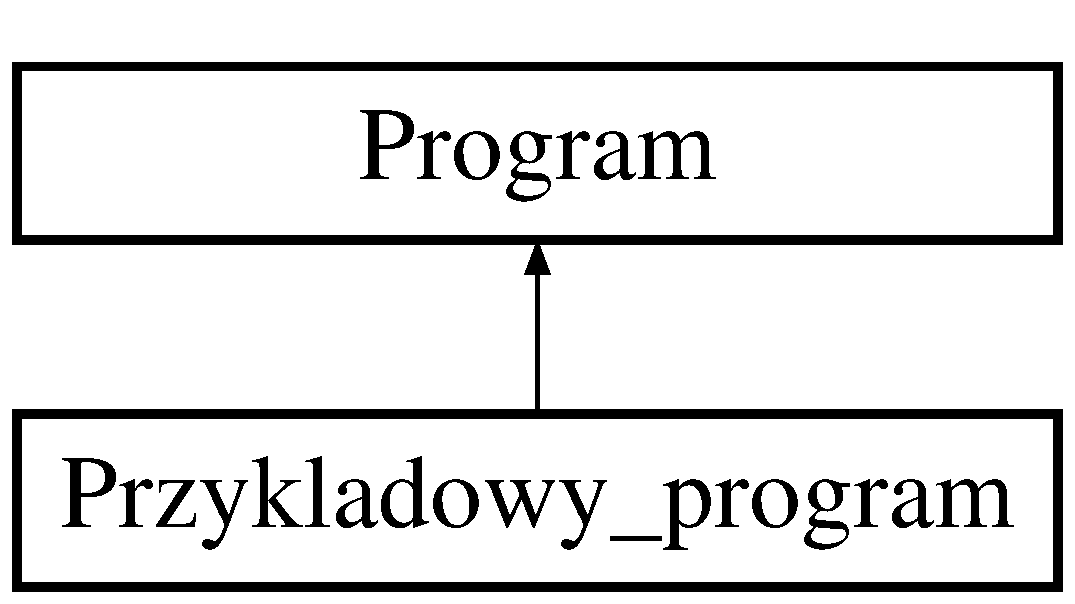
\includegraphics[height=2.000000cm]{class_program}
\end{center}
\end{figure}
\subsection*{Public Member Functions}
\begin{DoxyCompactItemize}
\item 
bool \hyperlink{class_program_aaef7fcaf64830eb231cbb9e887d705af}{zapisz\-\_\-dane} (char $\ast$nazwa)
\begin{DoxyCompactList}\small\item\em Metoda zapisz\-\_\-dane. \end{DoxyCompactList}\item 
void \hyperlink{class_program_a060ea3afebf696152d50135d20856e5a}{wypisz\-\_\-dane} ()
\begin{DoxyCompactList}\small\item\em Metoda wypisz\-\_\-dane. \end{DoxyCompactList}\item 
bool \hyperlink{class_program_ab5441e0e8ecd02ffeada4d77aaad2726}{porownaj\-\_\-dane} (char $\ast$nazwa)
\begin{DoxyCompactList}\small\item\em Metoda porownaj\-\_\-dane. \end{DoxyCompactList}\item 
virtual bool \hyperlink{class_program_ac396401ba5cade863d0e6acb727bec4e}{wykonaj\-\_\-program} ()
\begin{DoxyCompactList}\small\item\em Metoda wykonaj\-\_\-program. \end{DoxyCompactList}\item 
clock\-\_\-t \hyperlink{class_program_ab68c69977637eb8cc05a57e176a21986}{zacznij\-\_\-pomiar\-\_\-czasu} ()
\begin{DoxyCompactList}\small\item\em Metoda zacznij\-\_\-pomiar\-\_\-czasu. \end{DoxyCompactList}\item 
clock\-\_\-t \hyperlink{class_program_a3515568f8df7224bfd8fd8b7b76ab0ba}{zakoncz\-\_\-pomiar\-\_\-czasu} ()
\begin{DoxyCompactList}\small\item\em Metoda zakoncz\-\_\-pomiar\-\_\-czasu. \end{DoxyCompactList}\end{DoxyCompactItemize}
\subsection*{Public Attributes}
\begin{DoxyCompactItemize}
\item 
\hypertarget{class_program_ac27fc896de0e4c87cc6a17290c0930ef}{\hyperlink{class_tablica}{Tablica} {\bfseries dane}}\label{class_program_ac27fc896de0e4c87cc6a17290c0930ef}

\item 
clock\-\_\-t \hyperlink{class_program_a8cdcc795adc329732f41b399044d0a5b}{czas\-\_\-rozpoczecia}
\begin{DoxyCompactList}\small\item\em Zmienna czas\-\_\-rozpoczecia. \end{DoxyCompactList}\item 
fstream \hyperlink{class_program_a532ceacb1d70da66142bab96a3eb0753}{plik\-\_\-wejsciowy}
\begin{DoxyCompactList}\small\item\em Zmienna plik\-\_\-wejsciowy. \end{DoxyCompactList}\item 
fstream \hyperlink{class_program_aaa305591a4333d799c8d353f3072d8e0}{plik\-\_\-wyjsciowy}
\begin{DoxyCompactList}\small\item\em Zmienna plik\-\_\-wyjsciowy. \end{DoxyCompactList}\end{DoxyCompactItemize}


\subsection{Detailed Description}
Klasa \hyperlink{class_program}{Program}. 

Klasa odpowiedzialana za wykonanie operacji zwiazanych z pomiarem czasu oraz obsluge plikow, na ktorych wykonywane sa dzialania. Jest to klasa bazowa dla poszczegolnych algorytmow, ktorych metody moga zostac nadpisane. 

\subsection{Member Function Documentation}
\hypertarget{class_program_ab5441e0e8ecd02ffeada4d77aaad2726}{\index{Program@{Program}!porownaj\-\_\-dane@{porownaj\-\_\-dane}}
\index{porownaj\-\_\-dane@{porownaj\-\_\-dane}!Program@{Program}}
\subsubsection[{porownaj\-\_\-dane}]{\setlength{\rightskip}{0pt plus 5cm}bool Program\-::porownaj\-\_\-dane (
\begin{DoxyParamCaption}
\item[{char $\ast$}]{nazwa}
\end{DoxyParamCaption}
)}}\label{class_program_ab5441e0e8ecd02ffeada4d77aaad2726}


Metoda porownaj\-\_\-dane. 

Metoda porownujaca otrzymane dane ze spodziewanym wynikiem. 
\begin{DoxyParams}[1]{Parameters}
\mbox{\tt in}  & {\em Wskaznik} & do pliku zawierajacego poprawny wynik obliczen. \\
\hline
\end{DoxyParams}
\begin{DoxyReturn}{Returns}
Metoda zwraca wartosc true jesli udalo sie otworzyc odpowiedni plik i dane sa zgodne z wynikajacymi z obliczen. W przeciwynym wypadku metoda zwraca wartosc false i wyswietla odpowiedni komunikat. 
\end{DoxyReturn}
\hypertarget{class_program_ac396401ba5cade863d0e6acb727bec4e}{\index{Program@{Program}!wykonaj\-\_\-program@{wykonaj\-\_\-program}}
\index{wykonaj\-\_\-program@{wykonaj\-\_\-program}!Program@{Program}}
\subsubsection[{wykonaj\-\_\-program}]{\setlength{\rightskip}{0pt plus 5cm}bool Program\-::wykonaj\-\_\-program (
\begin{DoxyParamCaption}
{}
\end{DoxyParamCaption}
)\hspace{0.3cm}{\ttfamily [virtual]}}}\label{class_program_ac396401ba5cade863d0e6acb727bec4e}


Metoda wykonaj\-\_\-program. 

Metoda wykonujaca glowny algorytm programu. \begin{DoxyReturn}{Returns}
Metoda zwraca wartosc false jesli nie zostala nadpisana inna metoda z klasy dziedziczacej i wyswietla odpowiedni komunikat. 
\end{DoxyReturn}
\hypertarget{class_program_a060ea3afebf696152d50135d20856e5a}{\index{Program@{Program}!wypisz\-\_\-dane@{wypisz\-\_\-dane}}
\index{wypisz\-\_\-dane@{wypisz\-\_\-dane}!Program@{Program}}
\subsubsection[{wypisz\-\_\-dane}]{\setlength{\rightskip}{0pt plus 5cm}void Program\-::wypisz\-\_\-dane (
\begin{DoxyParamCaption}
{}
\end{DoxyParamCaption}
)}}\label{class_program_a060ea3afebf696152d50135d20856e5a}


Metoda wypisz\-\_\-dane. 

Metoda, ktora wypisuje przetworzone dane na standardowym wyjsciu. \hypertarget{class_program_ab68c69977637eb8cc05a57e176a21986}{\index{Program@{Program}!zacznij\-\_\-pomiar\-\_\-czasu@{zacznij\-\_\-pomiar\-\_\-czasu}}
\index{zacznij\-\_\-pomiar\-\_\-czasu@{zacznij\-\_\-pomiar\-\_\-czasu}!Program@{Program}}
\subsubsection[{zacznij\-\_\-pomiar\-\_\-czasu}]{\setlength{\rightskip}{0pt plus 5cm}clock\-\_\-t Program\-::zacznij\-\_\-pomiar\-\_\-czasu (
\begin{DoxyParamCaption}
{}
\end{DoxyParamCaption}
)}}\label{class_program_ab68c69977637eb8cc05a57e176a21986}


Metoda zacznij\-\_\-pomiar\-\_\-czasu. 

Metoda zapisujaca czas rozpoczecia pomiaru w odpowiednim polu klasy. \begin{DoxyReturn}{Returns}
Zwraca odczytany czas. 
\end{DoxyReturn}
\hypertarget{class_program_a3515568f8df7224bfd8fd8b7b76ab0ba}{\index{Program@{Program}!zakoncz\-\_\-pomiar\-\_\-czasu@{zakoncz\-\_\-pomiar\-\_\-czasu}}
\index{zakoncz\-\_\-pomiar\-\_\-czasu@{zakoncz\-\_\-pomiar\-\_\-czasu}!Program@{Program}}
\subsubsection[{zakoncz\-\_\-pomiar\-\_\-czasu}]{\setlength{\rightskip}{0pt plus 5cm}clock\-\_\-t Program\-::zakoncz\-\_\-pomiar\-\_\-czasu (
\begin{DoxyParamCaption}
{}
\end{DoxyParamCaption}
)}}\label{class_program_a3515568f8df7224bfd8fd8b7b76ab0ba}


Metoda zakoncz\-\_\-pomiar\-\_\-czasu. 

\begin{DoxyReturn}{Returns}
Zwraca dlugosc czasu wykonania programu (ilosc taktow zegara podzielona przez preskaler). 
\end{DoxyReturn}
\hypertarget{class_program_aaef7fcaf64830eb231cbb9e887d705af}{\index{Program@{Program}!zapisz\-\_\-dane@{zapisz\-\_\-dane}}
\index{zapisz\-\_\-dane@{zapisz\-\_\-dane}!Program@{Program}}
\subsubsection[{zapisz\-\_\-dane}]{\setlength{\rightskip}{0pt plus 5cm}bool Program\-::zapisz\-\_\-dane (
\begin{DoxyParamCaption}
\item[{char $\ast$}]{nazwa}
\end{DoxyParamCaption}
)}}\label{class_program_aaef7fcaf64830eb231cbb9e887d705af}


Metoda zapisz\-\_\-dane. 


\begin{DoxyParams}[1]{Parameters}
\mbox{\tt in}  & {\em Wskaznik} & do nazwy pliku, pod ktorym ma zostac zapisany strumien wyjsciowy. \\
\hline
\end{DoxyParams}
\begin{DoxyReturn}{Returns}
Zwraca 
\end{DoxyReturn}


\subsection{Member Data Documentation}
\hypertarget{class_program_a8cdcc795adc329732f41b399044d0a5b}{\index{Program@{Program}!czas\-\_\-rozpoczecia@{czas\-\_\-rozpoczecia}}
\index{czas\-\_\-rozpoczecia@{czas\-\_\-rozpoczecia}!Program@{Program}}
\subsubsection[{czas\-\_\-rozpoczecia}]{\setlength{\rightskip}{0pt plus 5cm}clock\-\_\-t Program\-::czas\-\_\-rozpoczecia}}\label{class_program_a8cdcc795adc329732f41b399044d0a5b}


Zmienna czas\-\_\-rozpoczecia. 

Zawiera czas w ktorym zaczal wykonywac sie wlasciwy kod algorytmu (liczony od momentu uruchomienia programu). Do tej danej porownywany jest czas zakoczenia wykonywania algorytmu. \hypertarget{class_program_a532ceacb1d70da66142bab96a3eb0753}{\index{Program@{Program}!plik\-\_\-wejsciowy@{plik\-\_\-wejsciowy}}
\index{plik\-\_\-wejsciowy@{plik\-\_\-wejsciowy}!Program@{Program}}
\subsubsection[{plik\-\_\-wejsciowy}]{\setlength{\rightskip}{0pt plus 5cm}fstream Program\-::plik\-\_\-wejsciowy}}\label{class_program_a532ceacb1d70da66142bab96a3eb0753}


Zmienna plik\-\_\-wejsciowy. 

Zmienna przedstawiajaca otwarty plik jako strumien danych. \hypertarget{class_program_aaa305591a4333d799c8d353f3072d8e0}{\index{Program@{Program}!plik\-\_\-wyjsciowy@{plik\-\_\-wyjsciowy}}
\index{plik\-\_\-wyjsciowy@{plik\-\_\-wyjsciowy}!Program@{Program}}
\subsubsection[{plik\-\_\-wyjsciowy}]{\setlength{\rightskip}{0pt plus 5cm}fstream Program\-::plik\-\_\-wyjsciowy}}\label{class_program_aaa305591a4333d799c8d353f3072d8e0}


Zmienna plik\-\_\-wyjsciowy. 

Zmienna przedstawiajaca strumien danych po wykonaniu wlasiwego algorytmu. 

The documentation for this class was generated from the following files\-:\begin{DoxyCompactItemize}
\item 
inc/\hyperlink{program_8hh}{program.\-hh}\item 
src/\hyperlink{program_8cpp}{program.\-cpp}\end{DoxyCompactItemize}

\hypertarget{class_przykladowy__program}{\section{Przykladowy\+\_\+program Class Reference}
\label{class_przykladowy__program}\index{Przykladowy\+\_\+program@{Przykladowy\+\_\+program}}
}


Klasa \hyperlink{class_przykladowy__program}{Przykladowy\+\_\+program}.  




{\ttfamily \#include $<$przykladowy\+\_\+program.\+hh$>$}

Inheritance diagram for Przykladowy\+\_\+program\+:\begin{figure}[H]
\begin{center}
\leavevmode
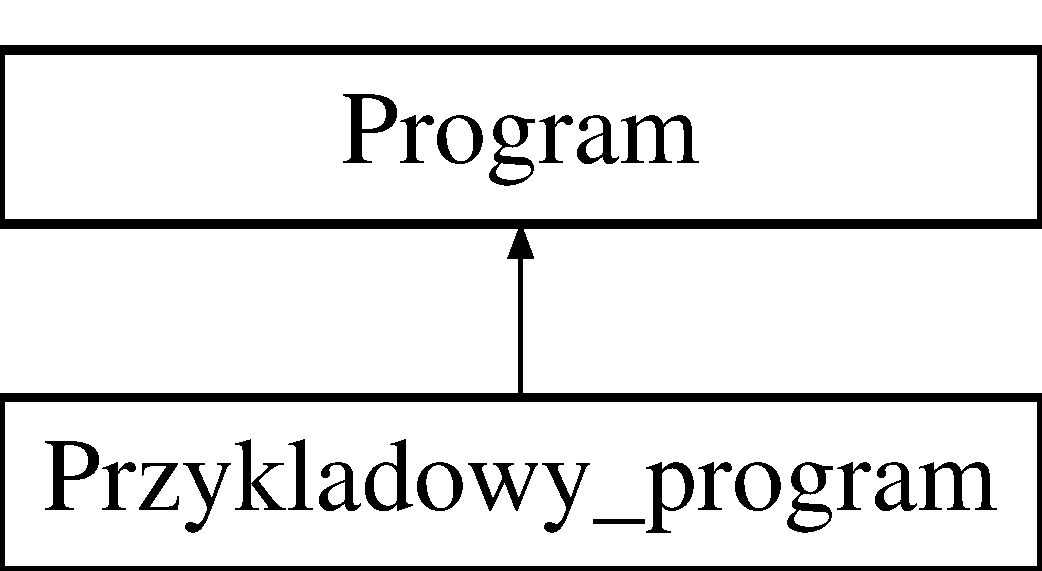
\includegraphics[height=2.000000cm]{class_przykladowy__program}
\end{center}
\end{figure}
\subsection*{Public Member Functions}
\begin{DoxyCompactItemize}
\item 
bool \hyperlink{class_przykladowy__program_a4215d5b5562be2a26f601dec4d4f6501}{wykonaj\+\_\+program} (\hyperlink{class_tablica}{Tablica} \&\hyperlink{class_program_ac27fc896de0e4c87cc6a17290c0930ef}{dane})
\begin{DoxyCompactList}\small\item\em Metoda wykonaj\+\_\+program. \end{DoxyCompactList}\item 
bool \hyperlink{class_przykladowy__program_a01cb33d6717d2dfd159f4607b7c8269f}{stworz\+\_\+plik\+\_\+testowy} (int ilosc, char $\ast$nazwa)
\begin{DoxyCompactList}\small\item\em Metoda stworz\+\_\+plik\+\_\+testowy. \end{DoxyCompactList}\end{DoxyCompactItemize}
\subsection*{Additional Inherited Members}


\subsection{Detailed Description}
Klasa \hyperlink{class_przykladowy__program}{Przykladowy\+\_\+program}. 

Klasa odpowiedzialna za zastapienie metody klasy \hyperlink{class_program}{Program} wlasna. Docelowo jest to plik w ktorym bedzie znajdowac sie wlasciwy algorytm. 

\subsection{Member Function Documentation}
\hypertarget{class_przykladowy__program_a01cb33d6717d2dfd159f4607b7c8269f}{\index{Przykladowy\+\_\+program@{Przykladowy\+\_\+program}!stworz\+\_\+plik\+\_\+testowy@{stworz\+\_\+plik\+\_\+testowy}}
\index{stworz\+\_\+plik\+\_\+testowy@{stworz\+\_\+plik\+\_\+testowy}!Przykladowy\+\_\+program@{Przykladowy\+\_\+program}}
\subsubsection[{stworz\+\_\+plik\+\_\+testowy}]{\setlength{\rightskip}{0pt plus 5cm}bool Przykladowy\+\_\+program\+::stworz\+\_\+plik\+\_\+testowy (
\begin{DoxyParamCaption}
\item[{int}]{ilosc, }
\item[{char $\ast$}]{nazwa}
\end{DoxyParamCaption}
)\hspace{0.3cm}{\ttfamily [virtual]}}}\label{class_przykladowy__program_a01cb33d6717d2dfd159f4607b7c8269f}


Metoda stworz\+\_\+plik\+\_\+testowy. 

Metoda zapisujaca do pliku dane, ktore moga byc wykorzystywane przy dzialaniu konkretnego programu jako dane wejsciowe. 

Reimplemented from \hyperlink{class_program_a7fa8a33fb88f842b544e6d65c23022c3}{Program}.

\hypertarget{class_przykladowy__program_a4215d5b5562be2a26f601dec4d4f6501}{\index{Przykladowy\+\_\+program@{Przykladowy\+\_\+program}!wykonaj\+\_\+program@{wykonaj\+\_\+program}}
\index{wykonaj\+\_\+program@{wykonaj\+\_\+program}!Przykladowy\+\_\+program@{Przykladowy\+\_\+program}}
\subsubsection[{wykonaj\+\_\+program}]{\setlength{\rightskip}{0pt plus 5cm}bool Przykladowy\+\_\+program\+::wykonaj\+\_\+program (
\begin{DoxyParamCaption}
\item[{{\bf Tablica} \&}]{dane}
\end{DoxyParamCaption}
)}}\label{class_przykladowy__program_a4215d5b5562be2a26f601dec4d4f6501}


Metoda wykonaj\+\_\+program. 

Wykonuje czynnosci zgodne z zadanym algorytmem. 

The documentation for this class was generated from the following files\+:\begin{DoxyCompactItemize}
\item 
inc/\hyperlink{przykladowy__program_8hh}{przykladowy\+\_\+program.\+hh}\item 
src/\hyperlink{przykladowy__program_8cpp}{przykladowy\+\_\+program.\+cpp}\end{DoxyCompactItemize}

\hypertarget{class_stos__lub__kolejka}{\section{Stos\+\_\+lub\+\_\+kolejka$<$ typ, struktura $>$ Class Template Reference}
\label{class_stos__lub__kolejka}\index{Stos\+\_\+lub\+\_\+kolejka$<$ typ, struktura $>$@{Stos\+\_\+lub\+\_\+kolejka$<$ typ, struktura $>$}}
}


Klasa \hyperlink{class_stos__lub__kolejka}{Stos\+\_\+lub\+\_\+kolejka}.  




{\ttfamily \#include $<$kolejka\+\_\+stos.\+hh$>$}

\subsection*{Public Member Functions}
\begin{DoxyCompactItemize}
\item 
bool \hyperlink{class_stos__lub__kolejka_ae3ed97741c87e68ab828989140b6cf6e}{is\+\_\+empty} ()
\begin{DoxyCompactList}\small\item\em Metoda is\+\_\+empty. \end{DoxyCompactList}\item 
int \hyperlink{class_stos__lub__kolejka_a11ef2a4fc9973ec37aa5a28a2ea824ba}{size} ()
\begin{DoxyCompactList}\small\item\em Metoda size. \end{DoxyCompactList}\item 
void \hyperlink{class_stos__lub__kolejka_ad514d78e27f4eed981eff2321e6b503e}{push} (typ element)
\begin{DoxyCompactList}\small\item\em Metoda push. \end{DoxyCompactList}\item 
bool \hyperlink{class_stos__lub__kolejka_a3d511f510942d9f0ac52a1fedee9100b}{pop} ()
\begin{DoxyCompactList}\small\item\em Metoda pop. \end{DoxyCompactList}\item 
void \hyperlink{class_stos__lub__kolejka_ae7859d2564799375487398f366342d54}{wypisz} ()
\begin{DoxyCompactList}\small\item\em Metoda wypisz. \end{DoxyCompactList}\item 
typ \hyperlink{class_stos__lub__kolejka_a9ed2032a0653ee8ae9d0111dcd3816d7}{front} ()
\begin{DoxyCompactList}\small\item\em Metoda front. \end{DoxyCompactList}\item 
\hypertarget{class_stos__lub__kolejka_aeb0f6510fab4df741b7b2316929f3704}{\hyperlink{class_stos__lub__kolejka_aeb0f6510fab4df741b7b2316929f3704}{Stos\+\_\+lub\+\_\+kolejka} ()}\label{class_stos__lub__kolejka_aeb0f6510fab4df741b7b2316929f3704}

\begin{DoxyCompactList}\small\item\em Konstruktor \hyperlink{class_stos__lub__kolejka}{Stos\+\_\+lub\+\_\+kolejka}. \end{DoxyCompactList}\end{DoxyCompactItemize}
\subsection*{Public Attributes}
\begin{DoxyCompactItemize}
\item 
int \hyperlink{class_stos__lub__kolejka_a1a93d8c833d23302598430ddf03a3d06}{ilosc\+\_\+danych}
\begin{DoxyCompactList}\small\item\em Zmienna ilosc\+\_\+danych. \end{DoxyCompactList}\item 
int \hyperlink{class_stos__lub__kolejka_a73d579d36148bb5047d5d6693aa69b57}{wielkosc\+\_\+tablicy}
\begin{DoxyCompactList}\small\item\em Zmienna wielkosc tablicy. \end{DoxyCompactList}\end{DoxyCompactItemize}
\subsection*{Private Attributes}
\begin{DoxyCompactItemize}
\item 
typ $\ast$ \hyperlink{class_stos__lub__kolejka_ad4f12e59b183d738823c43eb99c7bd37}{stos}
\begin{DoxyCompactList}\small\item\em Zmienna stos. \end{DoxyCompactList}\end{DoxyCompactItemize}


\subsection{Detailed Description}
\subsubsection*{template$<$class typ, rodzaj\+\_\+struktury struktura$>$class Stos\+\_\+lub\+\_\+kolejka$<$ typ, struktura $>$}

Klasa \hyperlink{class_stos__lub__kolejka}{Stos\+\_\+lub\+\_\+kolejka}. 

Jest to klasa moga funkcjonowac jako kolejka lub stos w zaleznosci od sposobu wywolania. 

\subsection{Member Function Documentation}
\hypertarget{class_stos__lub__kolejka_a9ed2032a0653ee8ae9d0111dcd3816d7}{\index{Stos\+\_\+lub\+\_\+kolejka@{Stos\+\_\+lub\+\_\+kolejka}!front@{front}}
\index{front@{front}!Stos\+\_\+lub\+\_\+kolejka@{Stos\+\_\+lub\+\_\+kolejka}}
\subsubsection[{front}]{\setlength{\rightskip}{0pt plus 5cm}template$<$class typ , rodzaj\+\_\+struktury struktura$>$ typ {\bf Stos\+\_\+lub\+\_\+kolejka}$<$ typ, struktura $>$\+::front (
\begin{DoxyParamCaption}
{}
\end{DoxyParamCaption}
)}}\label{class_stos__lub__kolejka_a9ed2032a0653ee8ae9d0111dcd3816d7}


Metoda front. 

Metoda zwracajaca element, ktory zostanie usuniety w pierwszej kolejnosci ze stosu lub kolejki. \hypertarget{class_stos__lub__kolejka_ae3ed97741c87e68ab828989140b6cf6e}{\index{Stos\+\_\+lub\+\_\+kolejka@{Stos\+\_\+lub\+\_\+kolejka}!is\+\_\+empty@{is\+\_\+empty}}
\index{is\+\_\+empty@{is\+\_\+empty}!Stos\+\_\+lub\+\_\+kolejka@{Stos\+\_\+lub\+\_\+kolejka}}
\subsubsection[{is\+\_\+empty}]{\setlength{\rightskip}{0pt plus 5cm}template$<$class typ , rodzaj\+\_\+struktury struktura$>$ bool {\bf Stos\+\_\+lub\+\_\+kolejka}$<$ typ, struktura $>$\+::is\+\_\+empty (
\begin{DoxyParamCaption}
{}
\end{DoxyParamCaption}
)}}\label{class_stos__lub__kolejka_ae3ed97741c87e68ab828989140b6cf6e}


Metoda is\+\_\+empty. 

Metoda sprawdzajaca czy stos/kolejka jest pusty/a \hypertarget{class_stos__lub__kolejka_a3d511f510942d9f0ac52a1fedee9100b}{\index{Stos\+\_\+lub\+\_\+kolejka@{Stos\+\_\+lub\+\_\+kolejka}!pop@{pop}}
\index{pop@{pop}!Stos\+\_\+lub\+\_\+kolejka@{Stos\+\_\+lub\+\_\+kolejka}}
\subsubsection[{pop}]{\setlength{\rightskip}{0pt plus 5cm}template$<$class typ , rodzaj\+\_\+struktury struktura$>$ bool {\bf Stos\+\_\+lub\+\_\+kolejka}$<$ typ, struktura $>$\+::pop (
\begin{DoxyParamCaption}
{}
\end{DoxyParamCaption}
)}}\label{class_stos__lub__kolejka_a3d511f510942d9f0ac52a1fedee9100b}


Metoda pop. 

Metoda zdejmujaca element ze stosu/kolejki \hypertarget{class_stos__lub__kolejka_ad514d78e27f4eed981eff2321e6b503e}{\index{Stos\+\_\+lub\+\_\+kolejka@{Stos\+\_\+lub\+\_\+kolejka}!push@{push}}
\index{push@{push}!Stos\+\_\+lub\+\_\+kolejka@{Stos\+\_\+lub\+\_\+kolejka}}
\subsubsection[{push}]{\setlength{\rightskip}{0pt plus 5cm}template$<$class typ , rodzaj\+\_\+struktury struktura$>$ void {\bf Stos\+\_\+lub\+\_\+kolejka}$<$ typ, struktura $>$\+::push (
\begin{DoxyParamCaption}
\item[{typ}]{element}
\end{DoxyParamCaption}
)}}\label{class_stos__lub__kolejka_ad514d78e27f4eed981eff2321e6b503e}


Metoda push. 

Metoda dodajaca element na stos/do kolejki \hypertarget{class_stos__lub__kolejka_a11ef2a4fc9973ec37aa5a28a2ea824ba}{\index{Stos\+\_\+lub\+\_\+kolejka@{Stos\+\_\+lub\+\_\+kolejka}!size@{size}}
\index{size@{size}!Stos\+\_\+lub\+\_\+kolejka@{Stos\+\_\+lub\+\_\+kolejka}}
\subsubsection[{size}]{\setlength{\rightskip}{0pt plus 5cm}template$<$class typ , rodzaj\+\_\+struktury struktura$>$ int {\bf Stos\+\_\+lub\+\_\+kolejka}$<$ typ, struktura $>$\+::size (
\begin{DoxyParamCaption}
{}
\end{DoxyParamCaption}
)}}\label{class_stos__lub__kolejka_a11ef2a4fc9973ec37aa5a28a2ea824ba}


Metoda size. 

Metoda podajaca rozmiar stosu/kolejki \hypertarget{class_stos__lub__kolejka_ae7859d2564799375487398f366342d54}{\index{Stos\+\_\+lub\+\_\+kolejka@{Stos\+\_\+lub\+\_\+kolejka}!wypisz@{wypisz}}
\index{wypisz@{wypisz}!Stos\+\_\+lub\+\_\+kolejka@{Stos\+\_\+lub\+\_\+kolejka}}
\subsubsection[{wypisz}]{\setlength{\rightskip}{0pt plus 5cm}template$<$class typ , rodzaj\+\_\+struktury struktura$>$ void {\bf Stos\+\_\+lub\+\_\+kolejka}$<$ typ, struktura $>$\+::wypisz (
\begin{DoxyParamCaption}
{}
\end{DoxyParamCaption}
)}}\label{class_stos__lub__kolejka_ae7859d2564799375487398f366342d54}


Metoda wypisz. 

Metoda wypisujaca stos/kolejke 

\subsection{Member Data Documentation}
\hypertarget{class_stos__lub__kolejka_a1a93d8c833d23302598430ddf03a3d06}{\index{Stos\+\_\+lub\+\_\+kolejka@{Stos\+\_\+lub\+\_\+kolejka}!ilosc\+\_\+danych@{ilosc\+\_\+danych}}
\index{ilosc\+\_\+danych@{ilosc\+\_\+danych}!Stos\+\_\+lub\+\_\+kolejka@{Stos\+\_\+lub\+\_\+kolejka}}
\subsubsection[{ilosc\+\_\+danych}]{\setlength{\rightskip}{0pt plus 5cm}template$<$class typ , rodzaj\+\_\+struktury struktura$>$ int {\bf Stos\+\_\+lub\+\_\+kolejka}$<$ typ, struktura $>$\+::ilosc\+\_\+danych}}\label{class_stos__lub__kolejka_a1a93d8c833d23302598430ddf03a3d06}


Zmienna ilosc\+\_\+danych. 

Zmienna przechowujaca informacje o ilosci danych znajdujacych sie w tablicy \hypertarget{class_stos__lub__kolejka_ad4f12e59b183d738823c43eb99c7bd37}{\index{Stos\+\_\+lub\+\_\+kolejka@{Stos\+\_\+lub\+\_\+kolejka}!stos@{stos}}
\index{stos@{stos}!Stos\+\_\+lub\+\_\+kolejka@{Stos\+\_\+lub\+\_\+kolejka}}
\subsubsection[{stos}]{\setlength{\rightskip}{0pt plus 5cm}template$<$class typ , rodzaj\+\_\+struktury struktura$>$ typ$\ast$ {\bf Stos\+\_\+lub\+\_\+kolejka}$<$ typ, struktura $>$\+::stos\hspace{0.3cm}{\ttfamily [private]}}}\label{class_stos__lub__kolejka_ad4f12e59b183d738823c43eb99c7bd37}


Zmienna stos. 

Wskaznik do tablicy w ktorej przechowywane sa dane. \hypertarget{class_stos__lub__kolejka_a73d579d36148bb5047d5d6693aa69b57}{\index{Stos\+\_\+lub\+\_\+kolejka@{Stos\+\_\+lub\+\_\+kolejka}!wielkosc\+\_\+tablicy@{wielkosc\+\_\+tablicy}}
\index{wielkosc\+\_\+tablicy@{wielkosc\+\_\+tablicy}!Stos\+\_\+lub\+\_\+kolejka@{Stos\+\_\+lub\+\_\+kolejka}}
\subsubsection[{wielkosc\+\_\+tablicy}]{\setlength{\rightskip}{0pt plus 5cm}template$<$class typ , rodzaj\+\_\+struktury struktura$>$ int {\bf Stos\+\_\+lub\+\_\+kolejka}$<$ typ, struktura $>$\+::wielkosc\+\_\+tablicy}}\label{class_stos__lub__kolejka_a73d579d36148bb5047d5d6693aa69b57}


Zmienna wielkosc tablicy. 

Zmienna okreslajaca wielkosc tablicy z danymi 

The documentation for this class was generated from the following file\+:\begin{DoxyCompactItemize}
\item 
inc/\hyperlink{kolejka__stos_8hh}{kolejka\+\_\+stos.\+hh}\end{DoxyCompactItemize}

\hypertarget{class_tablica}{\section{Tablica Class Reference}
\label{class_tablica}\index{Tablica@{Tablica}}
}


Klasa \hyperlink{class_program}{Program}.  




{\ttfamily \#include $<$tablica.\-hh$>$}

\subsection*{Public Member Functions}
\begin{DoxyCompactItemize}
\item 
\hyperlink{class_tablica}{Tablica} \hyperlink{class_tablica_a2d776cbdc02ed70b045b2c680bfdb695}{operator=} (const \hyperlink{class_tablica}{Tablica} dane)
\begin{DoxyCompactList}\small\item\em Przeciazenie operatora =. \end{DoxyCompactList}\item 
\hypertarget{class_tablica_a5f484e7b0478e1ff9b62e894f9d7b28d}{\hyperlink{class_tablica_a5f484e7b0478e1ff9b62e894f9d7b28d}{Tablica} ()}\label{class_tablica_a5f484e7b0478e1ff9b62e894f9d7b28d}

\begin{DoxyCompactList}\small\item\em Przeciazenie konstruktora bezparametrycznego. \end{DoxyCompactList}\item 
\hypertarget{class_tablica_aee4b66a81059b6ef1881909cd9f344b4}{\hyperlink{class_tablica_aee4b66a81059b6ef1881909cd9f344b4}{Tablica} (int ilosc)}\label{class_tablica_aee4b66a81059b6ef1881909cd9f344b4}

\begin{DoxyCompactList}\small\item\em Przeciazenie konstruktora parametrycznego. \end{DoxyCompactList}\item 
bool \hyperlink{class_tablica_a3864d3f5d0a339a496136e3546e71759}{operator==} (const \hyperlink{class_tablica}{Tablica} dane)
\begin{DoxyCompactList}\small\item\em Przeciazenie operatora ==. \end{DoxyCompactList}\end{DoxyCompactItemize}
\subsection*{Public Attributes}
\begin{DoxyCompactItemize}
\item 
\begin{tabbing}
xx\=xx\=xx\=xx\=xx\=xx\=xx\=xx\=xx\=\kill
union \{\\
\hypertarget{union_tablica_1_1@0_a15feeb49d1b632313b0f85102261038d}{\>string $\ast$ {\bfseries napisy}\\
\hypertarget{union_tablica_1_1@0_a9c67bc855a20899cc0eb7086ec96a745}{\>double $\ast$ {\bfseries tablica}\\
\}; \\

\end{tabbing}\begin{DoxyCompactList}\small\item\em Zmienna tablica. \end{DoxyCompactList}\item 
string $\ast$ \hyperlink{class_tablica_a86dbdede5dfd94c3ff34e35213ba4ff2}{klucze}
\begin{DoxyCompactList}\small\item\em Zmienna klucze. \end{DoxyCompactList}\item 
int \hyperlink{class_tablica_ab0d3e4210dc8a77e0f1c75834084c077}{dlugosc\-\_\-tablicy}
\begin{DoxyCompactList}\small\item\em Zmienna dlugosc\-\_\-tablicy. \end{DoxyCompactList}\end{DoxyCompactItemize}


\subsection{Detailed Description}
Klasa \hyperlink{class_program}{Program}. 

Klasa w ktorej przechowywane sa dane oraz zawierajaca niektore metody na nich wykonywane. 

\subsection{Member Function Documentation}
\hypertarget{class_tablica_a2d776cbdc02ed70b045b2c680bfdb695}{\index{Tablica@{Tablica}!operator=@{operator=}}
\index{operator=@{operator=}!Tablica@{Tablica}}
\subsubsection[{operator=}]{\setlength{\rightskip}{0pt plus 5cm}{\bf Tablica} Tablica\-::operator= (
\begin{DoxyParamCaption}
\item[{const {\bf Tablica}}]{dane}
\end{DoxyParamCaption}
)}}\label{class_tablica_a2d776cbdc02ed70b045b2c680bfdb695}


Przeciazenie operatora =. 

Wykonuje przepisanie wartosci z jednej Tablicy do drugiej \hypertarget{class_tablica_a3864d3f5d0a339a496136e3546e71759}{\index{Tablica@{Tablica}!operator==@{operator==}}
\index{operator==@{operator==}!Tablica@{Tablica}}
\subsubsection[{operator==}]{\setlength{\rightskip}{0pt plus 5cm}bool Tablica\-::operator== (
\begin{DoxyParamCaption}
\item[{const {\bf Tablica}}]{dane}
\end{DoxyParamCaption}
)}}\label{class_tablica_a3864d3f5d0a339a496136e3546e71759}


Przeciazenie operatora ==. 

/return Zwraca wartosc true jesli Tablice sa zgodne. W przeciwnym wypadku wartosc false. 

\subsection{Member Data Documentation}
\hypertarget{class_tablica_a52448ef22993bdc85475e124fe89e76a}{\subsubsection[{"@1}]{\setlength{\rightskip}{0pt plus 5cm}union \{ ... \} }}\label{class_tablica_a52448ef22993bdc85475e124fe89e76a}


Zmienna tablica. 

Zawiera wskaznik do dynamicznie tworzonej tablicy, w ktorej przechowywane sa dane uprzednio wczytane z podanego pliku. \hypertarget{class_tablica_ab0d3e4210dc8a77e0f1c75834084c077}{\index{Tablica@{Tablica}!dlugosc\-\_\-tablicy@{dlugosc\-\_\-tablicy}}
\index{dlugosc\-\_\-tablicy@{dlugosc\-\_\-tablicy}!Tablica@{Tablica}}
\subsubsection[{dlugosc\-\_\-tablicy}]{\setlength{\rightskip}{0pt plus 5cm}int Tablica\-::dlugosc\-\_\-tablicy}}\label{class_tablica_ab0d3e4210dc8a77e0f1c75834084c077}


Zmienna dlugosc\-\_\-tablicy. 

Zawiera liczbe swiadczaco o dlugosci utworzonej tablicy dynamicznej. \hypertarget{class_tablica_a86dbdede5dfd94c3ff34e35213ba4ff2}{\index{Tablica@{Tablica}!klucze@{klucze}}
\index{klucze@{klucze}!Tablica@{Tablica}}
\subsubsection[{klucze}]{\setlength{\rightskip}{0pt plus 5cm}string$\ast$ Tablica\-::klucze}}\label{class_tablica_a86dbdede5dfd94c3ff34e35213ba4ff2}


Zmienna klucze. 

Zawiera klucze do danych znajdujacych sie w tablicy. W najprostrzym wypadku dane powinny byc wpisane w tej samej kolejnosci. 

The documentation for this class was generated from the following file\-:\begin{DoxyCompactItemize}
\item 
inc/\hyperlink{tablica_8hh}{tablica.\-hh}\end{DoxyCompactItemize}

\hypertarget{class_tablica__hash}{\section{Tablica\+\_\+hash$<$ typ, klucz, dana $>$ Class Template Reference}
\label{class_tablica__hash}\index{Tablica\+\_\+hash$<$ typ, klucz, dana $>$@{Tablica\+\_\+hash$<$ typ, klucz, dana $>$}}
}


Klasa \hyperlink{class_tablica__hash}{Tablica\+\_\+hash}.  




{\ttfamily \#include $<$tab\+\_\+hash.\+hh$>$}

\subsection*{Public Member Functions}
\begin{DoxyCompactItemize}
\item 
bool \hyperlink{class_tablica__hash_a2f4ff5542110d6b6aa1cebcab857e888}{dodaj} (klucz haslo, klucz haslo2, dana wartosc)
\begin{DoxyCompactList}\small\item\em Metoda dodaj. \end{DoxyCompactList}\item 
bool \hyperlink{class_tablica__hash_ad0f14e672fb51ccb1a7f4398b756fa3a}{znajdz1} (klucz haslo)
\begin{DoxyCompactList}\small\item\em Metoda znajdz1. \end{DoxyCompactList}\item 
bool \hyperlink{class_tablica__hash_a45cb10776d07c4269518cd065e514c3b}{znajdz2} (klucz haslo, klucz haslo2)
\begin{DoxyCompactList}\small\item\em Metoda znajdz2. \end{DoxyCompactList}\item 
typ $\ast$ \hyperlink{class_tablica__hash_a6b751df11a6e2674c44e09a14551d1f5}{zwroc\+\_\+element} (klucz haslo)
\begin{DoxyCompactList}\small\item\em Metoda pobierz. \end{DoxyCompactList}\item 
\hypertarget{class_tablica__hash_a71cfb5cb24ff2639b880da0b6126f256}{\hyperlink{class_tablica__hash_a71cfb5cb24ff2639b880da0b6126f256}{Tablica\+\_\+hash} ()}\label{class_tablica__hash_a71cfb5cb24ff2639b880da0b6126f256}

\begin{DoxyCompactList}\small\item\em Konstruktor tablicy z hashowaniem. \end{DoxyCompactList}\item 
int \hyperlink{class_tablica__hash_a3bf2052f56f9167232ba2030540366ad}{zlicz\+\_\+elementy} ()
\begin{DoxyCompactList}\small\item\em Metoda zlicz. \end{DoxyCompactList}\item 
bool \hyperlink{class_tablica__hash_a7f05fe199025e1b1227f0e6002ae4277}{usun\+\_\+element} (klucz haslo, klucz haslo2)
\begin{DoxyCompactList}\small\item\em usun\+\_\+element \end{DoxyCompactList}\item 
bool \hyperlink{class_tablica__hash_a3bb7f336108b94763baaa39177ace487}{usun\+\_\+klucz} (klucz haslo)
\begin{DoxyCompactList}\small\item\em usun\+\_\+klucz \end{DoxyCompactList}\item 
typ $\ast$ \hyperlink{class_tablica__hash_a95d61a05450373b45703ddf3235861b7}{nastepny} (typ $\ast$element)
\begin{DoxyCompactList}\small\item\em nastepny \end{DoxyCompactList}\item 
void \hyperlink{class_tablica__hash_a69240feec1270aee65f3a8f608a64a97}{wypisz} ()
\begin{DoxyCompactList}\small\item\em wypisz \end{DoxyCompactList}\end{DoxyCompactItemize}
\subsection*{Private Member Functions}
\begin{DoxyCompactItemize}
\item 
int \hyperlink{class_tablica__hash_ae66e0710cf8d52bd94d234c38c7a98bb}{funkcja\+\_\+hash} (klucz haslo)
\begin{DoxyCompactList}\small\item\em funkcja\+\_\+hash \end{DoxyCompactList}\end{DoxyCompactItemize}
\subsection*{Private Attributes}
\begin{DoxyCompactItemize}
\item 
typ $\ast$$\ast$ \hyperlink{class_tablica__hash_a066b590b47cc28b38a6fabfb061ab7ca}{tablica}
\begin{DoxyCompactList}\small\item\em tablica \end{DoxyCompactList}\item 
int \hyperlink{class_tablica__hash_a749b330424ccf3ebca23b708a65e619c}{ilosc\+\_\+elementow}
\begin{DoxyCompactList}\small\item\em Zmienna ilosc\+\_\+elementow. \end{DoxyCompactList}\end{DoxyCompactItemize}


\subsection{Detailed Description}
\subsubsection*{template$<$class typ, class klucz, class dana$>$class Tablica\+\_\+hash$<$ typ, klucz, dana $>$}

Klasa \hyperlink{class_tablica__hash}{Tablica\+\_\+hash}. 

Klasa tworzaca tablice z hashowanie i wykonujaca na niej czynnosci zwiazane z zapisem i odczytem. 

\subsection{Member Function Documentation}
\hypertarget{class_tablica__hash_a2f4ff5542110d6b6aa1cebcab857e888}{\index{Tablica\+\_\+hash@{Tablica\+\_\+hash}!dodaj@{dodaj}}
\index{dodaj@{dodaj}!Tablica\+\_\+hash@{Tablica\+\_\+hash}}
\subsubsection[{dodaj}]{\setlength{\rightskip}{0pt plus 5cm}template$<$class typ , class klucz , class dana $>$ bool {\bf Tablica\+\_\+hash}$<$ typ, klucz, dana $>$\+::dodaj (
\begin{DoxyParamCaption}
\item[{klucz}]{haslo, }
\item[{klucz}]{haslo2, }
\item[{dana}]{wartosc}
\end{DoxyParamCaption}
)}}\label{class_tablica__hash_a2f4ff5542110d6b6aa1cebcab857e888}


Metoda dodaj. 

Metoda dodajaca element na odpowiednie miejsce w tabeli/liscie. Jesli element jest dodawany na liscie to umieszcza sie go w sposob posortowany. \hypertarget{class_tablica__hash_ae66e0710cf8d52bd94d234c38c7a98bb}{\index{Tablica\+\_\+hash@{Tablica\+\_\+hash}!funkcja\+\_\+hash@{funkcja\+\_\+hash}}
\index{funkcja\+\_\+hash@{funkcja\+\_\+hash}!Tablica\+\_\+hash@{Tablica\+\_\+hash}}
\subsubsection[{funkcja\+\_\+hash}]{\setlength{\rightskip}{0pt plus 5cm}template$<$class typ , class klucz , class dana $>$ int {\bf Tablica\+\_\+hash}$<$ typ, klucz, dana $>$\+::funkcja\+\_\+hash (
\begin{DoxyParamCaption}
\item[{klucz}]{haslo}
\end{DoxyParamCaption}
)\hspace{0.3cm}{\ttfamily [private]}}}\label{class_tablica__hash_ae66e0710cf8d52bd94d234c38c7a98bb}


funkcja\+\_\+hash 

Metoda wykonujaca przydzielenie odpowiedniej komorki tablicy dla danego elementu \hypertarget{class_tablica__hash_a95d61a05450373b45703ddf3235861b7}{\index{Tablica\+\_\+hash@{Tablica\+\_\+hash}!nastepny@{nastepny}}
\index{nastepny@{nastepny}!Tablica\+\_\+hash@{Tablica\+\_\+hash}}
\subsubsection[{nastepny}]{\setlength{\rightskip}{0pt plus 5cm}template$<$class typ , class klucz , class dana $>$ typ $\ast$ {\bf Tablica\+\_\+hash}$<$ typ, klucz, dana $>$\+::nastepny (
\begin{DoxyParamCaption}
\item[{typ $\ast$}]{element}
\end{DoxyParamCaption}
)}}\label{class_tablica__hash_a95d61a05450373b45703ddf3235861b7}


nastepny 

Metoda zwracajaca wskaznik do nastepnego w tablicy z hashowanie elementu o tym samym kluczu. \hypertarget{class_tablica__hash_a7f05fe199025e1b1227f0e6002ae4277}{\index{Tablica\+\_\+hash@{Tablica\+\_\+hash}!usun\+\_\+element@{usun\+\_\+element}}
\index{usun\+\_\+element@{usun\+\_\+element}!Tablica\+\_\+hash@{Tablica\+\_\+hash}}
\subsubsection[{usun\+\_\+element}]{\setlength{\rightskip}{0pt plus 5cm}template$<$class typ , class klucz , class dana $>$ bool {\bf Tablica\+\_\+hash}$<$ typ, klucz, dana $>$\+::usun\+\_\+element (
\begin{DoxyParamCaption}
\item[{klucz}]{haslo, }
\item[{klucz}]{haslo2}
\end{DoxyParamCaption}
)}}\label{class_tablica__hash_a7f05fe199025e1b1227f0e6002ae4277}


usun\+\_\+element 

Metoda usuwajaca element, o zadanych kluczach. \hypertarget{class_tablica__hash_a3bb7f336108b94763baaa39177ace487}{\index{Tablica\+\_\+hash@{Tablica\+\_\+hash}!usun\+\_\+klucz@{usun\+\_\+klucz}}
\index{usun\+\_\+klucz@{usun\+\_\+klucz}!Tablica\+\_\+hash@{Tablica\+\_\+hash}}
\subsubsection[{usun\+\_\+klucz}]{\setlength{\rightskip}{0pt plus 5cm}template$<$class typ , class klucz , class dana $>$ bool {\bf Tablica\+\_\+hash}$<$ typ, klucz, dana $>$\+::usun\+\_\+klucz (
\begin{DoxyParamCaption}
\item[{klucz}]{haslo}
\end{DoxyParamCaption}
)}}\label{class_tablica__hash_a3bb7f336108b94763baaa39177ace487}


usun\+\_\+klucz 

Metoda usuwajaca wszystkie elementy o zadanym kluczu. \hypertarget{class_tablica__hash_a69240feec1270aee65f3a8f608a64a97}{\index{Tablica\+\_\+hash@{Tablica\+\_\+hash}!wypisz@{wypisz}}
\index{wypisz@{wypisz}!Tablica\+\_\+hash@{Tablica\+\_\+hash}}
\subsubsection[{wypisz}]{\setlength{\rightskip}{0pt plus 5cm}template$<$class typ , class klucz , class dana $>$ void {\bf Tablica\+\_\+hash}$<$ typ, klucz, dana $>$\+::wypisz (
\begin{DoxyParamCaption}
{}
\end{DoxyParamCaption}
)}}\label{class_tablica__hash_a69240feec1270aee65f3a8f608a64a97}


wypisz 

Metoda wypisujaca cala tablice z hashowanie. \hypertarget{class_tablica__hash_a3bf2052f56f9167232ba2030540366ad}{\index{Tablica\+\_\+hash@{Tablica\+\_\+hash}!zlicz\+\_\+elementy@{zlicz\+\_\+elementy}}
\index{zlicz\+\_\+elementy@{zlicz\+\_\+elementy}!Tablica\+\_\+hash@{Tablica\+\_\+hash}}
\subsubsection[{zlicz\+\_\+elementy}]{\setlength{\rightskip}{0pt plus 5cm}template$<$class typ , class klucz , class dana $>$ int {\bf Tablica\+\_\+hash}$<$ typ, klucz, dana $>$\+::zlicz\+\_\+elementy (
\begin{DoxyParamCaption}
{}
\end{DoxyParamCaption}
)}}\label{class_tablica__hash_a3bf2052f56f9167232ba2030540366ad}


Metoda zlicz. 

\begin{DoxyReturn}{Returns}
Metoda zwraca ilosc elementow wpisanych do struktury. 
\end{DoxyReturn}
\hypertarget{class_tablica__hash_ad0f14e672fb51ccb1a7f4398b756fa3a}{\index{Tablica\+\_\+hash@{Tablica\+\_\+hash}!znajdz1@{znajdz1}}
\index{znajdz1@{znajdz1}!Tablica\+\_\+hash@{Tablica\+\_\+hash}}
\subsubsection[{znajdz1}]{\setlength{\rightskip}{0pt plus 5cm}template$<$class typ , class klucz , class dana $>$ bool {\bf Tablica\+\_\+hash}$<$ typ, klucz, dana $>$\+::znajdz1 (
\begin{DoxyParamCaption}
\item[{klucz}]{haslo}
\end{DoxyParamCaption}
)}}\label{class_tablica__hash_ad0f14e672fb51ccb1a7f4398b756fa3a}


Metoda znajdz1. 

Metoda znajdujaca zadany element. \begin{DoxyReturn}{Returns}
Zwraca true jesli znaleziono element i false jesli nie uda�o sie znalezc elementu. 
\end{DoxyReturn}
\hypertarget{class_tablica__hash_a45cb10776d07c4269518cd065e514c3b}{\index{Tablica\+\_\+hash@{Tablica\+\_\+hash}!znajdz2@{znajdz2}}
\index{znajdz2@{znajdz2}!Tablica\+\_\+hash@{Tablica\+\_\+hash}}
\subsubsection[{znajdz2}]{\setlength{\rightskip}{0pt plus 5cm}template$<$class typ , class klucz , class dana $>$ bool {\bf Tablica\+\_\+hash}$<$ typ, klucz, dana $>$\+::znajdz2 (
\begin{DoxyParamCaption}
\item[{klucz}]{haslo, }
\item[{klucz}]{haslo2}
\end{DoxyParamCaption}
)}}\label{class_tablica__hash_a45cb10776d07c4269518cd065e514c3b}


Metoda znajdz2. 

Metoda znajdujaca zadany element. \begin{DoxyReturn}{Returns}
Zwraca true jesli znaleziono element i false jesli nie uda�o sie znalezc elementu. 
\end{DoxyReturn}
\hypertarget{class_tablica__hash_a6b751df11a6e2674c44e09a14551d1f5}{\index{Tablica\+\_\+hash@{Tablica\+\_\+hash}!zwroc\+\_\+element@{zwroc\+\_\+element}}
\index{zwroc\+\_\+element@{zwroc\+\_\+element}!Tablica\+\_\+hash@{Tablica\+\_\+hash}}
\subsubsection[{zwroc\+\_\+element}]{\setlength{\rightskip}{0pt plus 5cm}template$<$class typ , class klucz , class dana $>$ typ $\ast$ {\bf Tablica\+\_\+hash}$<$ typ, klucz, dana $>$\+::zwroc\+\_\+element (
\begin{DoxyParamCaption}
\item[{klucz}]{haslo}
\end{DoxyParamCaption}
)}}\label{class_tablica__hash_a6b751df11a6e2674c44e09a14551d1f5}


Metoda pobierz. 

Metoda znajdujaca zadany element. \begin{DoxyReturn}{Returns}
Zwraca element na liscie jesli taki istniej. Jesli nie to zwraca N\+U\+L\+L. 
\end{DoxyReturn}


\subsection{Member Data Documentation}
\hypertarget{class_tablica__hash_a749b330424ccf3ebca23b708a65e619c}{\index{Tablica\+\_\+hash@{Tablica\+\_\+hash}!ilosc\+\_\+elementow@{ilosc\+\_\+elementow}}
\index{ilosc\+\_\+elementow@{ilosc\+\_\+elementow}!Tablica\+\_\+hash@{Tablica\+\_\+hash}}
\subsubsection[{ilosc\+\_\+elementow}]{\setlength{\rightskip}{0pt plus 5cm}template$<$class typ , class klucz , class dana $>$ int {\bf Tablica\+\_\+hash}$<$ typ, klucz, dana $>$\+::ilosc\+\_\+elementow\hspace{0.3cm}{\ttfamily [private]}}}\label{class_tablica__hash_a749b330424ccf3ebca23b708a65e619c}


Zmienna ilosc\+\_\+elementow. 

Zmienna przechowuj�ca informacje o ilosci wpisanych elementow do struktury. \hypertarget{class_tablica__hash_a066b590b47cc28b38a6fabfb061ab7ca}{\index{Tablica\+\_\+hash@{Tablica\+\_\+hash}!tablica@{tablica}}
\index{tablica@{tablica}!Tablica\+\_\+hash@{Tablica\+\_\+hash}}
\subsubsection[{tablica}]{\setlength{\rightskip}{0pt plus 5cm}template$<$class typ , class klucz , class dana $>$ typ$\ast$$\ast$ {\bf Tablica\+\_\+hash}$<$ typ, klucz, dana $>$\+::tablica\hspace{0.3cm}{\ttfamily [private]}}}\label{class_tablica__hash_a066b590b47cc28b38a6fabfb061ab7ca}


tablica 

\hyperlink{class_tablica}{Tablica} wskaznikow na pocz�tki list elementow. Elementy zawieraja klucz i dane. 

The documentation for this class was generated from the following file\+:\begin{DoxyCompactItemize}
\item 
inc/\hyperlink{tab__hash_8hh}{tab\+\_\+hash.\+hh}\end{DoxyCompactItemize}

\chapter{File Documentation}
\hypertarget{benchmark_8hh}{\section{inc/benchmark.hh File Reference}
\label{benchmark_8hh}\index{inc/benchmark.\-hh@{inc/benchmark.\-hh}}
}


Plik zawierajacy deklaracje klasy benchmark.  


{\ttfamily \#include \char`\"{}program.\-hh\char`\"{}}\\*
\subsection*{Classes}
\begin{DoxyCompactItemize}
\item 
class \hyperlink{classbenchmark}{benchmark}
\begin{DoxyCompactList}\small\item\em Klasa benchmarek. \end{DoxyCompactList}\end{DoxyCompactItemize}


\subsection{Detailed Description}
Plik zawierajacy deklaracje klasy benchmark. 
\hypertarget{element_8hh}{\section{inc/element.hh File Reference}
\label{element_8hh}\index{inc/element.\+hh@{inc/element.\+hh}}
}


Plik zawierajacy definicje i deklaracje klasy \hyperlink{class_element}{Element}.  


\subsection*{Classes}
\begin{DoxyCompactItemize}
\item 
class \hyperlink{class_element}{Element$<$ klucz, wartosc $>$}
\begin{DoxyCompactList}\small\item\em Klasa \hyperlink{class_element}{Element}. \end{DoxyCompactList}\end{DoxyCompactItemize}


\subsection{Detailed Description}
Plik zawierajacy definicje i deklaracje klasy \hyperlink{class_element}{Element}. 


\hypertarget{graf_8hh}{\section{inc/graf.hh File Reference}
\label{graf_8hh}\index{inc/graf.\+hh@{inc/graf.\+hh}}
}


Plik zawierajacy klase \hyperlink{class_graf}{Graf}.  


{\ttfamily \#include $<$iostream$>$}\\*
{\ttfamily \#include $<$queue$>$}\\*
{\ttfamily \#include \char`\"{}element.\+hh\char`\"{}}\\*
{\ttfamily \#include \char`\"{}tab\+\_\+hash.\+hh\char`\"{}}\\*
{\ttfamily \#include \char`\"{}kolejka\+\_\+stos.\+hh\char`\"{}}\\*
{\ttfamily \#include \char`\"{}lista\+\_\+posortowana.\+hh\char`\"{}}\\*
{\ttfamily \#include \char`\"{}konfiguracja.\+hh\char`\"{}}\\*
\subsection*{Classes}
\begin{DoxyCompactItemize}
\item 
class \hyperlink{class_graf}{Graf$<$ krawedz, wierzcholek $>$}
\begin{DoxyCompactList}\small\item\em Klasa \hyperlink{class_graf}{Graf}. \end{DoxyCompactList}\end{DoxyCompactItemize}
\subsection*{Enumerations}
\begin{DoxyCompactItemize}
\item 
\hypertarget{graf_8hh_a21e872a06a76ee7bc1a0acb523f9fdee}{enum {\bfseries rodzaj\+\_\+przeszukiwania} \{ {\bfseries joj}, 
{\bfseries best\+\_\+first\+\_\+search}
 \}}\label{graf_8hh_a21e872a06a76ee7bc1a0acb523f9fdee}

\end{DoxyCompactItemize}


\subsection{Detailed Description}
Plik zawierajacy klase \hyperlink{class_graf}{Graf}. 


\hypertarget{kolejka__stos_8hh}{\section{inc/kolejka\+\_\+stos.hh File Reference}
\label{kolejka__stos_8hh}\index{inc/kolejka\+\_\+stos.\+hh@{inc/kolejka\+\_\+stos.\+hh}}
}


Plik zawierajacy deklaracje klasy \hyperlink{class_stos__lub__kolejka}{Stos\+\_\+lub\+\_\+kolejka}.  


{\ttfamily \#include $<$iostream$>$}\\*
{\ttfamily \#include \char`\"{}konfiguracja.\+hh\char`\"{}}\\*
\subsection*{Classes}
\begin{DoxyCompactItemize}
\item 
class \hyperlink{class_stos__lub__kolejka}{Stos\+\_\+lub\+\_\+kolejka$<$ typ, struktura $>$}
\begin{DoxyCompactList}\small\item\em Klasa \hyperlink{class_stos__lub__kolejka}{Stos\+\_\+lub\+\_\+kolejka}. \end{DoxyCompactList}\end{DoxyCompactItemize}
\subsection*{Enumerations}
\begin{DoxyCompactItemize}
\item 
\hypertarget{kolejka__stos_8hh_ac4ee52880299a21ae4131d3532bb1609}{enum {\bfseries rodzaj\+\_\+struktury} \{ {\bfseries L\+I\+F\+O}, 
{\bfseries F\+I\+F\+O}
 \}}\label{kolejka__stos_8hh_ac4ee52880299a21ae4131d3532bb1609}

\end{DoxyCompactItemize}


\subsection{Detailed Description}
Plik zawierajacy deklaracje klasy \hyperlink{class_stos__lub__kolejka}{Stos\+\_\+lub\+\_\+kolejka}. 


\hypertarget{komunikacja_8hh}{\section{inc/komunikacja.hh File Reference}
\label{komunikacja_8hh}\index{inc/komunikacja.\+hh@{inc/komunikacja.\+hh}}
}


Plik zawierajacy deklaracje klasy \hyperlink{class_komunikacja}{Komunikacja}.  


{\ttfamily \#include $<$string$>$}\\*
{\ttfamily \#include \char`\"{}tablica.\+hh\char`\"{}}\\*
\subsection*{Classes}
\begin{DoxyCompactItemize}
\item 
class \hyperlink{class_komunikacja}{Komunikacja}
\begin{DoxyCompactList}\small\item\em Klasa \hyperlink{class_komunikacja}{Komunikacja}. \end{DoxyCompactList}\end{DoxyCompactItemize}


\subsection{Detailed Description}
Plik zawierajacy deklaracje klasy \hyperlink{class_komunikacja}{Komunikacja}. 


\hypertarget{program_8hh}{\section{inc/program.hh File Reference}
\label{program_8hh}\index{inc/program.\+hh@{inc/program.\+hh}}
}


Plik zawierajacy deklaracje klasy \hyperlink{class_program}{Program}.  


{\ttfamily \#include $<$fstream$>$}\\*
{\ttfamily \#include $<$ctime$>$}\\*
{\ttfamily \#include $<$cstdio$>$}\\*
{\ttfamily \#include \char`\"{}tablica.\+hh\char`\"{}}\\*
\subsection*{Classes}
\begin{DoxyCompactItemize}
\item 
class \hyperlink{class_program}{Program}
\begin{DoxyCompactList}\small\item\em Klasa \hyperlink{class_program}{Program}. \end{DoxyCompactList}\end{DoxyCompactItemize}


\subsection{Detailed Description}
Plik zawierajacy deklaracje klasy \hyperlink{class_program}{Program}. 


\hypertarget{przykladowy__program_8hh}{\section{inc/przykladowy\+\_\+program.hh File Reference}
\label{przykladowy__program_8hh}\index{inc/przykladowy\+\_\+program.\+hh@{inc/przykladowy\+\_\+program.\+hh}}
}


Plik zawierajacy deklaracje klasy \hyperlink{class_przykladowy__program}{Przykladowy\+\_\+program}.  


{\ttfamily \#include \char`\"{}program.\+hh\char`\"{}}\\*
{\ttfamily \#include \char`\"{}tablica.\+hh\char`\"{}}\\*
\subsection*{Classes}
\begin{DoxyCompactItemize}
\item 
class \hyperlink{class_przykladowy__program}{Przykladowy\+\_\+program}
\begin{DoxyCompactList}\small\item\em Klasa \hyperlink{class_przykladowy__program}{Przykladowy\+\_\+program}. \end{DoxyCompactList}\end{DoxyCompactItemize}


\subsection{Detailed Description}
Plik zawierajacy deklaracje klasy \hyperlink{class_przykladowy__program}{Przykladowy\+\_\+program}. 


\hypertarget{tab__hash_8hh}{\section{inc/tab\-\_\-hash.hh File Reference}
\label{tab__hash_8hh}\index{inc/tab\-\_\-hash.\-hh@{inc/tab\-\_\-hash.\-hh}}
}


Plik zawierajacy klase \hyperlink{class_tablica__hash}{Tablica\-\_\-hash}.  


{\ttfamily \#include $<$cmath$>$}\\*
{\ttfamily \#include $<$typeinfo$>$}\\*
{\ttfamily \#include \char`\"{}konfiguracja.\-hh\char`\"{}}\\*
\subsection*{Classes}
\begin{DoxyCompactItemize}
\item 
class \hyperlink{class_tablica__hash}{Tablica\-\_\-hash$<$ typ, klucz, dana $>$}
\begin{DoxyCompactList}\small\item\em Klasa \hyperlink{class_tablica__hash}{Tablica\-\_\-hash}. \end{DoxyCompactList}\end{DoxyCompactItemize}


\subsection{Detailed Description}
Plik zawierajacy klase \hyperlink{class_tablica__hash}{Tablica\-\_\-hash}. 
\hypertarget{tablica_8hh}{\section{inc/tablica.hh File Reference}
\label{tablica_8hh}\index{inc/tablica.\+hh@{inc/tablica.\+hh}}
}


Plik zawierajacy deklaracje klasy \hyperlink{class_tablica}{Tablica}.  


{\ttfamily \#include $<$string$>$}\\*
\subsection*{Classes}
\begin{DoxyCompactItemize}
\item 
class \hyperlink{class_tablica}{Tablica}
\begin{DoxyCompactList}\small\item\em Klasa \hyperlink{class_program}{Program}. \end{DoxyCompactList}\end{DoxyCompactItemize}


\subsection{Detailed Description}
Plik zawierajacy deklaracje klasy \hyperlink{class_tablica}{Tablica}. 


\hypertarget{benchmark_8cpp}{\section{src/benchmark.cpp File Reference}
\label{benchmark_8cpp}\index{src/benchmark.\+cpp@{src/benchmark.\+cpp}}
}


Plik zawierajacy definicje metod klasy benchmark.  


{\ttfamily \#include $<$iostream$>$}\\*
{\ttfamily \#include $<$ctime$>$}\\*
{\ttfamily \#include $<$cstdlib$>$}\\*
{\ttfamily \#include $<$string$>$}\\*
{\ttfamily \#include $<$sstream$>$}\\*
{\ttfamily \#include \char`\"{}przykladowy\+\_\+program.\+hh\char`\"{}}\\*
{\ttfamily \#include \char`\"{}benchmark.\+hh\char`\"{}}\\*
{\ttfamily \#include \char`\"{}komunikacja.\+hh\char`\"{}}\\*
{\ttfamily \#include \char`\"{}konfiguracja.\+hh\char`\"{}}\\*
{\ttfamily \#include \char`\"{}tab\+\_\+hash.\+hh\char`\"{}}\\*
{\ttfamily \#include \char`\"{}element.\+hh\char`\"{}}\\*


\subsection{Detailed Description}
Plik zawierajacy definicje metod klasy benchmark. 


\hypertarget{komunikacja_8cpp}{\section{src/komunikacja.cpp File Reference}
\label{komunikacja_8cpp}\index{src/komunikacja.\-cpp@{src/komunikacja.\-cpp}}
}


Plik zawierajacy definicje metod klasy \hyperlink{class_komunikacja}{Komunikacja}.  


{\ttfamily \#include $<$iostream$>$}\\*
{\ttfamily \#include $<$string$>$}\\*
{\ttfamily \#include $<$cstring$>$}\\*
{\ttfamily \#include $<$fstream$>$}\\*
{\ttfamily \#include $<$cctype$>$}\\*
{\ttfamily \#include $<$sstream$>$}\\*
{\ttfamily \#include \char`\"{}komunikacja.\-hh\char`\"{}}\\*


\subsection{Detailed Description}
Plik zawierajacy definicje metod klasy \hyperlink{class_komunikacja}{Komunikacja}. 
\hypertarget{main_8cpp}{\section{src/main.cpp File Reference}
\label{main_8cpp}\index{src/main.\+cpp@{src/main.\+cpp}}
}


Plik zawierajacy glowna funkcje programu wykonujacego benchmark algorytmu.  


{\ttfamily \#include $<$iostream$>$}\\*
{\ttfamily \#include \char`\"{}komunikacja.\+hh\char`\"{}}\\*
{\ttfamily \#include \char`\"{}benchmark.\+hh\char`\"{}}\\*
\subsection*{Functions}
\begin{DoxyCompactItemize}
\item 
int \hyperlink{main_8cpp_a840291bc02cba5474a4cb46a9b9566fe}{main} (void)
\begin{DoxyCompactList}\small\item\em Glowna funkcja programu. \end{DoxyCompactList}\end{DoxyCompactItemize}


\subsection{Detailed Description}
Plik zawierajacy glowna funkcje programu wykonujacego benchmark algorytmu. 



\subsection{Function Documentation}
\hypertarget{main_8cpp_a840291bc02cba5474a4cb46a9b9566fe}{\index{main.\+cpp@{main.\+cpp}!main@{main}}
\index{main@{main}!main.\+cpp@{main.\+cpp}}
\subsubsection[{main}]{\setlength{\rightskip}{0pt plus 5cm}int main (
\begin{DoxyParamCaption}
\item[{void}]{}
\end{DoxyParamCaption}
)}}\label{main_8cpp_a840291bc02cba5474a4cb46a9b9566fe}


Glowna funkcja programu. 

Funkcja wykonujaca benchmark zadanego algorytmu na podstawie czasu wykonywania operacji. 
\hypertarget{program_8cpp}{\section{src/program.cpp File Reference}
\label{program_8cpp}\index{src/program.\-cpp@{src/program.\-cpp}}
}


Plik zawierajacy definicje metod klasy \hyperlink{class_program}{Program}.  


{\ttfamily \#include $<$fstream$>$}\\*
{\ttfamily \#include $<$iostream$>$}\\*
{\ttfamily \#include $<$sstream$>$}\\*
{\ttfamily \#include $<$string$>$}\\*
{\ttfamily \#include $<$cstdio$>$}\\*
{\ttfamily \#include $<$ctime$>$}\\*
{\ttfamily \#include \char`\"{}program.\-hh\char`\"{}}\\*
{\ttfamily \#include \char`\"{}operacje.\-hh\char`\"{}}\\*
{\ttfamily \#include \char`\"{}komunikacja.\-hh\char`\"{}}\\*


\subsection{Detailed Description}
Plik zawierajacy definicje metod klasy \hyperlink{class_program}{Program}. 
\hypertarget{przykladowy__program_8cpp}{\section{src/przykladowy\+\_\+program.cpp File Reference}
\label{przykladowy__program_8cpp}\index{src/przykladowy\+\_\+program.\+cpp@{src/przykladowy\+\_\+program.\+cpp}}
}


Plik zawierajacy definicje metod klasy \hyperlink{class_przykladowy__program}{Przykladowy\+\_\+program}.  


{\ttfamily \#include $<$iostream$>$}\\*
{\ttfamily \#include $<$string$>$}\\*
{\ttfamily \#include $<$cstdlib$>$}\\*
{\ttfamily \#include $<$ctime$>$}\\*
{\ttfamily \#include \char`\"{}program.\+hh\char`\"{}}\\*
{\ttfamily \#include \char`\"{}przykladowy\+\_\+program.\+hh\char`\"{}}\\*
{\ttfamily \#include \char`\"{}tab\+\_\+hash.\+hh\char`\"{}}\\*
{\ttfamily \#include \char`\"{}konfiguracja.\+hh\char`\"{}}\\*
{\ttfamily \#include \char`\"{}plansza.\+hh\char`\"{}}\\*


\subsection{Detailed Description}
Plik zawierajacy definicje metod klasy \hyperlink{class_przykladowy__program}{Przykladowy\+\_\+program}. 


%--- End generated contents ---

% Index
\newpage
\phantomsection
\addcontentsline{toc}{chapter}{Index}
\printindex

\end{document}
